% Options for packages loaded elsewhere
\PassOptionsToPackage{unicode}{hyperref}
\PassOptionsToPackage{hyphens}{url}
%
\documentclass[
]{article}
\usepackage{amsmath,amssymb}
\usepackage{iftex}
\ifPDFTeX
  \usepackage[T1]{fontenc}
  \usepackage[utf8]{inputenc}
  \usepackage{textcomp} % provide euro and other symbols
\else % if luatex or xetex
  \usepackage{unicode-math} % this also loads fontspec
  \defaultfontfeatures{Scale=MatchLowercase}
  \defaultfontfeatures[\rmfamily]{Ligatures=TeX,Scale=1}
\fi
\usepackage{lmodern}
\ifPDFTeX\else
  % xetex/luatex font selection
\fi
% Use upquote if available, for straight quotes in verbatim environments
\IfFileExists{upquote.sty}{\usepackage{upquote}}{}
\IfFileExists{microtype.sty}{% use microtype if available
  \usepackage[]{microtype}
  \UseMicrotypeSet[protrusion]{basicmath} % disable protrusion for tt fonts
}{}
\makeatletter
\@ifundefined{KOMAClassName}{% if non-KOMA class
  \IfFileExists{parskip.sty}{%
    \usepackage{parskip}
  }{% else
    \setlength{\parindent}{0pt}
    \setlength{\parskip}{6pt plus 2pt minus 1pt}}
}{% if KOMA class
  \KOMAoptions{parskip=half}}
\makeatother
\usepackage{xcolor}
\usepackage[margin=1in]{geometry}
\usepackage{color}
\usepackage{fancyvrb}
\newcommand{\VerbBar}{|}
\newcommand{\VERB}{\Verb[commandchars=\\\{\}]}
\DefineVerbatimEnvironment{Highlighting}{Verbatim}{commandchars=\\\{\}}
% Add ',fontsize=\small' for more characters per line
\usepackage{framed}
\definecolor{shadecolor}{RGB}{248,248,248}
\newenvironment{Shaded}{\begin{snugshade}}{\end{snugshade}}
\newcommand{\AlertTok}[1]{\textcolor[rgb]{0.94,0.16,0.16}{#1}}
\newcommand{\AnnotationTok}[1]{\textcolor[rgb]{0.56,0.35,0.01}{\textbf{\textit{#1}}}}
\newcommand{\AttributeTok}[1]{\textcolor[rgb]{0.13,0.29,0.53}{#1}}
\newcommand{\BaseNTok}[1]{\textcolor[rgb]{0.00,0.00,0.81}{#1}}
\newcommand{\BuiltInTok}[1]{#1}
\newcommand{\CharTok}[1]{\textcolor[rgb]{0.31,0.60,0.02}{#1}}
\newcommand{\CommentTok}[1]{\textcolor[rgb]{0.56,0.35,0.01}{\textit{#1}}}
\newcommand{\CommentVarTok}[1]{\textcolor[rgb]{0.56,0.35,0.01}{\textbf{\textit{#1}}}}
\newcommand{\ConstantTok}[1]{\textcolor[rgb]{0.56,0.35,0.01}{#1}}
\newcommand{\ControlFlowTok}[1]{\textcolor[rgb]{0.13,0.29,0.53}{\textbf{#1}}}
\newcommand{\DataTypeTok}[1]{\textcolor[rgb]{0.13,0.29,0.53}{#1}}
\newcommand{\DecValTok}[1]{\textcolor[rgb]{0.00,0.00,0.81}{#1}}
\newcommand{\DocumentationTok}[1]{\textcolor[rgb]{0.56,0.35,0.01}{\textbf{\textit{#1}}}}
\newcommand{\ErrorTok}[1]{\textcolor[rgb]{0.64,0.00,0.00}{\textbf{#1}}}
\newcommand{\ExtensionTok}[1]{#1}
\newcommand{\FloatTok}[1]{\textcolor[rgb]{0.00,0.00,0.81}{#1}}
\newcommand{\FunctionTok}[1]{\textcolor[rgb]{0.13,0.29,0.53}{\textbf{#1}}}
\newcommand{\ImportTok}[1]{#1}
\newcommand{\InformationTok}[1]{\textcolor[rgb]{0.56,0.35,0.01}{\textbf{\textit{#1}}}}
\newcommand{\KeywordTok}[1]{\textcolor[rgb]{0.13,0.29,0.53}{\textbf{#1}}}
\newcommand{\NormalTok}[1]{#1}
\newcommand{\OperatorTok}[1]{\textcolor[rgb]{0.81,0.36,0.00}{\textbf{#1}}}
\newcommand{\OtherTok}[1]{\textcolor[rgb]{0.56,0.35,0.01}{#1}}
\newcommand{\PreprocessorTok}[1]{\textcolor[rgb]{0.56,0.35,0.01}{\textit{#1}}}
\newcommand{\RegionMarkerTok}[1]{#1}
\newcommand{\SpecialCharTok}[1]{\textcolor[rgb]{0.81,0.36,0.00}{\textbf{#1}}}
\newcommand{\SpecialStringTok}[1]{\textcolor[rgb]{0.31,0.60,0.02}{#1}}
\newcommand{\StringTok}[1]{\textcolor[rgb]{0.31,0.60,0.02}{#1}}
\newcommand{\VariableTok}[1]{\textcolor[rgb]{0.00,0.00,0.00}{#1}}
\newcommand{\VerbatimStringTok}[1]{\textcolor[rgb]{0.31,0.60,0.02}{#1}}
\newcommand{\WarningTok}[1]{\textcolor[rgb]{0.56,0.35,0.01}{\textbf{\textit{#1}}}}
\usepackage{graphicx}
\makeatletter
\def\maxwidth{\ifdim\Gin@nat@width>\linewidth\linewidth\else\Gin@nat@width\fi}
\def\maxheight{\ifdim\Gin@nat@height>\textheight\textheight\else\Gin@nat@height\fi}
\makeatother
% Scale images if necessary, so that they will not overflow the page
% margins by default, and it is still possible to overwrite the defaults
% using explicit options in \includegraphics[width, height, ...]{}
\setkeys{Gin}{width=\maxwidth,height=\maxheight,keepaspectratio}
% Set default figure placement to htbp
\makeatletter
\def\fps@figure{htbp}
\makeatother
\setlength{\emergencystretch}{3em} % prevent overfull lines
\providecommand{\tightlist}{%
  \setlength{\itemsep}{0pt}\setlength{\parskip}{0pt}}
\setcounter{secnumdepth}{5}
\ifLuaTeX
  \usepackage{selnolig}  % disable illegal ligatures
\fi
\IfFileExists{bookmark.sty}{\usepackage{bookmark}}{\usepackage{hyperref}}
\IfFileExists{xurl.sty}{\usepackage{xurl}}{} % add URL line breaks if available
\urlstyle{same}
\hypersetup{
  pdftitle={Data Science Salary Analysis},
  pdfauthor={Sue Susman, MEd, BSN, RN},
  hidelinks,
  pdfcreator={LaTeX via pandoc}}

\title{Data Science Salary Analysis}
\author{Sue Susman, MEd, BSN, RN}
\date{2023-07-06}

\begin{document}
\maketitle

{
\setcounter{tocdepth}{6}
\tableofcontents
}
\hypertarget{project-overview}{%
\section{Project Overview:}\label{project-overview}}

The CEO of the small, but rapidly expanding company I work for is
interested in adding a full-time data scientist to the staff. While the
company is in the US, there is a possibility for this position to be
remote for the right person. Factors to consider include rising salaries
in the recession, along with a highly competitive job market. My
research will explore salaries of data jobs in and out of the US. I will
attempt to identify trends and patterns in the data science job market,
including experience levels, location of companies, company sizes,
salary differences between hiring someone in the US vs.~someone outside
of the US.

\begin{Shaded}
\begin{Highlighting}[]
\FunctionTok{options}\NormalTok{(}\AttributeTok{repos =} \StringTok{"https://cran.rstudio.com/"}\NormalTok{)}
\end{Highlighting}
\end{Shaded}

\begin{Shaded}
\begin{Highlighting}[]
    \FunctionTok{install.packages}\NormalTok{(}\StringTok{"tidyverse"}\NormalTok{)}
\end{Highlighting}
\end{Shaded}

\begin{verbatim}
## 
## The downloaded binary packages are in
##  /var/folders/7w/vf_3wx5d6kq9bm2666hl7yy80000gn/T//RtmpZAhJKC/downloaded_packages
\end{verbatim}

\begin{Shaded}
\begin{Highlighting}[]
    \FunctionTok{install.packages}\NormalTok{(}\StringTok{"ggwordcloud"}\NormalTok{)}
\end{Highlighting}
\end{Shaded}

\begin{verbatim}
## 
## The downloaded binary packages are in
##  /var/folders/7w/vf_3wx5d6kq9bm2666hl7yy80000gn/T//RtmpZAhJKC/downloaded_packages
\end{verbatim}

\begin{Shaded}
\begin{Highlighting}[]
    \FunctionTok{install.packages}\NormalTok{(}\StringTok{"viridis"}\NormalTok{)}
\end{Highlighting}
\end{Shaded}

\begin{verbatim}
## 
## The downloaded binary packages are in
##  /var/folders/7w/vf_3wx5d6kq9bm2666hl7yy80000gn/T//RtmpZAhJKC/downloaded_packages
\end{verbatim}

\begin{Shaded}
\begin{Highlighting}[]
    \FunctionTok{install.packages}\NormalTok{(}\StringTok{"scales"}\NormalTok{)}
\end{Highlighting}
\end{Shaded}

\begin{verbatim}
## 
## The downloaded binary packages are in
##  /var/folders/7w/vf_3wx5d6kq9bm2666hl7yy80000gn/T//RtmpZAhJKC/downloaded_packages
\end{verbatim}

\begin{Shaded}
\begin{Highlighting}[]
    \FunctionTok{install.packages}\NormalTok{(}\StringTok{"dplyr"}\NormalTok{)}
\end{Highlighting}
\end{Shaded}

\begin{verbatim}
## 
## The downloaded binary packages are in
##  /var/folders/7w/vf_3wx5d6kq9bm2666hl7yy80000gn/T//RtmpZAhJKC/downloaded_packages
\end{verbatim}

\begin{Shaded}
\begin{Highlighting}[]
    \FunctionTok{library}\NormalTok{(tidyverse)}
\end{Highlighting}
\end{Shaded}

\begin{verbatim}
## -- Attaching core tidyverse packages ------------------------ tidyverse 2.0.0 --
## v dplyr     1.1.2     v readr     2.1.4
## v forcats   1.0.0     v stringr   1.5.0
## v ggplot2   3.4.2     v tibble    3.2.1
## v lubridate 1.9.2     v tidyr     1.3.0
## v purrr     1.0.1     
## -- Conflicts ------------------------------------------ tidyverse_conflicts() --
## x dplyr::filter() masks stats::filter()
## x dplyr::lag()    masks stats::lag()
## i Use the conflicted package (<http://conflicted.r-lib.org/>) to force all conflicts to become errors
\end{verbatim}

\begin{Shaded}
\begin{Highlighting}[]
    \FunctionTok{library}\NormalTok{(ggwordcloud)}
    \FunctionTok{library}\NormalTok{(viridis)}
\end{Highlighting}
\end{Shaded}

\begin{verbatim}
## Loading required package: viridisLite
\end{verbatim}

\begin{Shaded}
\begin{Highlighting}[]
    \FunctionTok{library}\NormalTok{(scales)}
\end{Highlighting}
\end{Shaded}

\begin{verbatim}
## 
## Attaching package: 'scales'
## 
## The following object is masked from 'package:viridis':
## 
##     viridis_pal
## 
## The following object is masked from 'package:purrr':
## 
##     discard
## 
## The following object is masked from 'package:readr':
## 
##     col_factor
\end{verbatim}

\begin{Shaded}
\begin{Highlighting}[]
    \FunctionTok{library}\NormalTok{(dplyr)}

    \FunctionTok{options}\NormalTok{(}\AttributeTok{repr.plot.width =} \DecValTok{15}\NormalTok{, }\AttributeTok{repr.plot.height =} \DecValTok{15}\NormalTok{)}
\end{Highlighting}
\end{Shaded}

\begin{Shaded}
\begin{Highlighting}[]
\CommentTok{\#Main Data set}
\NormalTok{salary\_df }\OtherTok{\textless{}{-}} \FunctionTok{read.csv}\NormalTok{(}\StringTok{"data.csv"}\NormalTok{)}

\CommentTok{\#Country codes Data set, used for cleaning later}
\NormalTok{iso\_df }\OtherTok{\textless{}{-}} \FunctionTok{read.csv}\NormalTok{(}\StringTok{"wikipedia{-}iso{-}country{-}codes.csv"}\NormalTok{)}
\end{Highlighting}
\end{Shaded}

Checking the dimensions of a dataframe can be useful for understanding
the size and structure of your data and for performing various
operations and analyses based on the number of rows and columns present.

\begin{Shaded}
\begin{Highlighting}[]
\FunctionTok{t}\NormalTok{(}\FunctionTok{t}\NormalTok{(}\FunctionTok{names}\NormalTok{(salary\_df))) }\CommentTok{\# In summary, the code transposes the column names of the data\_df dataframe and returns them as a column matrix to display the column names in a user friendly manner.}
\end{Highlighting}
\end{Shaded}

\begin{verbatim}
##       [,1]                
##  [1,] "X"                 
##  [2,] "work_year"         
##  [3,] "experience_level"  
##  [4,] "employment_type"   
##  [5,] "job_title"         
##  [6,] "salary"            
##  [7,] "salary_currency"   
##  [8,] "salary_in_usd"     
##  [9,] "employee_residence"
## [10,] "remote_ratio"      
## [11,] "company_location"  
## [12,] "company_size"
\end{verbatim}

\begin{Shaded}
\begin{Highlighting}[]
\CommentTok{\#Dimensions of the data frame}
\NormalTok{data\_dimensions }\OtherTok{\textless{}{-}} \FunctionTok{dim}\NormalTok{(salary\_df)}
\NormalTok{num\_rows }\OtherTok{\textless{}{-}}\NormalTok{ data\_dimensions[}\DecValTok{1}\NormalTok{]}
\NormalTok{num\_cols }\OtherTok{\textless{}{-}}\NormalTok{ data\_dimensions[}\DecValTok{2}\NormalTok{]}

\NormalTok{text }\OtherTok{\textless{}{-}} \FunctionTok{paste}\NormalTok{(}\StringTok{"There are"}\NormalTok{, num\_rows,}\StringTok{"Rows"}\NormalTok{, }\StringTok{"and"}\NormalTok{, num\_cols, }\StringTok{"Columns"}\NormalTok{, }\StringTok{"in this dataset"}\NormalTok{)}

\FunctionTok{print}\NormalTok{(text)}
\end{Highlighting}
\end{Shaded}

\begin{verbatim}
## [1] "There are 607 Rows and 12 Columns in this dataset"
\end{verbatim}

\begin{Shaded}
\begin{Highlighting}[]
\FunctionTok{head}\NormalTok{(salary\_df)  }\CommentTok{\#Displays the first couple of rows of the data frame}
\end{Highlighting}
\end{Shaded}

\begin{verbatim}
##   X work_year experience_level employment_type                  job_title
## 1 0      2020               MI              FT             Data Scientist
## 2 1      2020               SE              FT Machine Learning Scientist
## 3 2      2020               SE              FT          Big Data Engineer
## 4 3      2020               MI              FT       Product Data Analyst
## 5 4      2020               SE              FT  Machine Learning Engineer
## 6 5      2020               EN              FT               Data Analyst
##   salary salary_currency salary_in_usd employee_residence remote_ratio
## 1  70000             EUR         79833                 DE            0
## 2 260000             USD        260000                 JP            0
## 3  85000             GBP        109024                 GB           50
## 4  20000             USD         20000                 HN            0
## 5 150000             USD        150000                 US           50
## 6  72000             USD         72000                 US          100
##   company_location company_size
## 1               DE            L
## 2               JP            S
## 3               GB            M
## 4               HN            S
## 5               US            L
## 6               US            L
\end{verbatim}

\begin{Shaded}
\begin{Highlighting}[]
\FunctionTok{str}\NormalTok{(salary\_df)  }\CommentTok{\#Display list of columns and data types}
\end{Highlighting}
\end{Shaded}

\begin{verbatim}
## 'data.frame':    607 obs. of  12 variables:
##  $ X                 : int  0 1 2 3 4 5 6 7 8 9 ...
##  $ work_year         : int  2020 2020 2020 2020 2020 2020 2020 2020 2020 2020 ...
##  $ experience_level  : chr  "MI" "SE" "SE" "MI" ...
##  $ employment_type   : chr  "FT" "FT" "FT" "FT" ...
##  $ job_title         : chr  "Data Scientist" "Machine Learning Scientist" "Big Data Engineer" "Product Data Analyst" ...
##  $ salary            : int  70000 260000 85000 20000 150000 72000 190000 11000000 135000 125000 ...
##  $ salary_currency   : chr  "EUR" "USD" "GBP" "USD" ...
##  $ salary_in_usd     : int  79833 260000 109024 20000 150000 72000 190000 35735 135000 125000 ...
##  $ employee_residence: chr  "DE" "JP" "GB" "HN" ...
##  $ remote_ratio      : int  0 0 50 0 50 100 100 50 100 50 ...
##  $ company_location  : chr  "DE" "JP" "GB" "HN" ...
##  $ company_size      : chr  "L" "S" "M" "S" ...
\end{verbatim}

\begin{Shaded}
\begin{Highlighting}[]
\FunctionTok{summary}\NormalTok{(salary\_df)  }\CommentTok{\#Statistical summary of data }
\end{Highlighting}
\end{Shaded}

\begin{verbatim}
##        X           work_year    experience_level   employment_type   
##  Min.   :  0.0   Min.   :2020   Length:607         Length:607        
##  1st Qu.:151.5   1st Qu.:2021   Class :character   Class :character  
##  Median :303.0   Median :2022   Mode  :character   Mode  :character  
##  Mean   :303.0   Mean   :2021                                        
##  3rd Qu.:454.5   3rd Qu.:2022                                        
##  Max.   :606.0   Max.   :2022                                        
##   job_title             salary         salary_currency    salary_in_usd   
##  Length:607         Min.   :    4000   Length:607         Min.   :  2859  
##  Class :character   1st Qu.:   70000   Class :character   1st Qu.: 62726  
##  Mode  :character   Median :  115000   Mode  :character   Median :101570  
##                     Mean   :  324000                      Mean   :112298  
##                     3rd Qu.:  165000                      3rd Qu.:150000  
##                     Max.   :30400000                      Max.   :600000  
##  employee_residence  remote_ratio    company_location   company_size      
##  Length:607         Min.   :  0.00   Length:607         Length:607        
##  Class :character   1st Qu.: 50.00   Class :character   Class :character  
##  Mode  :character   Median :100.00   Mode  :character   Mode  :character  
##                     Mean   : 70.92                                        
##                     3rd Qu.:100.00                                        
##                     Max.   :100.00
\end{verbatim}

\begin{Shaded}
\begin{Highlighting}[]
\CommentTok{\# Checking for any NA values}
\FunctionTok{any}\NormalTok{(}\FunctionTok{is.na}\NormalTok{(salary\_df))}
\end{Highlighting}
\end{Shaded}

\begin{verbatim}
## [1] FALSE
\end{verbatim}

\begin{Shaded}
\begin{Highlighting}[]
\CommentTok{\#Checking for unique values per column}
\FunctionTok{library}\NormalTok{(dplyr)}
\NormalTok{salary\_df }\SpecialCharTok{\%\textgreater{}\%} 
  \FunctionTok{summarise}\NormalTok{(}
    \AttributeTok{work\_year =} \FunctionTok{n\_distinct}\NormalTok{(work\_year),}
    \AttributeTok{experience\_level =} \FunctionTok{n\_distinct}\NormalTok{(experience\_level),}
    \AttributeTok{employment\_type =} \FunctionTok{n\_distinct}\NormalTok{(employment\_type),}
    \AttributeTok{job\_title =} \FunctionTok{n\_distinct}\NormalTok{(job\_title),}
    \AttributeTok{salary =} \FunctionTok{n\_distinct}\NormalTok{(salary),}
    \AttributeTok{salary\_currency =} \FunctionTok{n\_distinct}\NormalTok{(salary\_currency),}
    \AttributeTok{salary\_in\_usd =} \FunctionTok{n\_distinct}\NormalTok{(salary\_in\_usd),}
    \AttributeTok{employee\_residence =} \FunctionTok{n\_distinct}\NormalTok{(employee\_residence),}
    \AttributeTok{remote\_ratio =} \FunctionTok{n\_distinct}\NormalTok{(remote\_ratio),}
    \AttributeTok{company\_location =} \FunctionTok{n\_distinct}\NormalTok{(company\_location),}
    \AttributeTok{company\_size =} \FunctionTok{n\_distinct}\NormalTok{(company\_size)}
\NormalTok{  )}
\end{Highlighting}
\end{Shaded}

\begin{verbatim}
##   work_year experience_level employment_type job_title salary salary_currency
## 1         3                4               4        50    272              17
##   salary_in_usd employee_residence remote_ratio company_location company_size
## 1           369                 57            3               50            3
\end{verbatim}

Cleaning the Data There are a few problems we need to fix: 1. The
columns experience\_level, employment\_type, employee\_residence,
company\_size and company\_location contain abbreviations that may not
be understood to some, we will rename the data contained in those
columns to more descriptive labels.¶

\begin{Shaded}
\begin{Highlighting}[]
\CommentTok{\#Renamed abbreviations for the experience\_level column}
\NormalTok{salary\_df}\SpecialCharTok{$}\NormalTok{experience\_level[salary\_df}\SpecialCharTok{$}\NormalTok{experience\_level }\SpecialCharTok{==} \StringTok{"SE"}\NormalTok{] }\OtherTok{\textless{}{-}} \StringTok{"Senior"}
\NormalTok{salary\_df}\SpecialCharTok{$}\NormalTok{experience\_level[salary\_df}\SpecialCharTok{$}\NormalTok{experience\_level }\SpecialCharTok{==} \StringTok{"MI"}\NormalTok{] }\OtherTok{\textless{}{-}} \StringTok{"Indermediate"}
\NormalTok{salary\_df}\SpecialCharTok{$}\NormalTok{experience\_level[salary\_df}\SpecialCharTok{$}\NormalTok{experience\_level }\SpecialCharTok{==} \StringTok{"EN"}\NormalTok{] }\OtherTok{\textless{}{-}} \StringTok{"Junior/Entry"}
\NormalTok{salary\_df}\SpecialCharTok{$}\NormalTok{experience\_level[salary\_df}\SpecialCharTok{$}\NormalTok{experience\_level }\SpecialCharTok{==} \StringTok{"EX"}\NormalTok{] }\OtherTok{\textless{}{-}} \StringTok{"Director/Executive"}

\CommentTok{\#Renamed abbreviations for the employment\_type column}
\NormalTok{salary\_df}\SpecialCharTok{$}\NormalTok{employment\_type[salary\_df}\SpecialCharTok{$}\NormalTok{employment\_type }\SpecialCharTok{==} \StringTok{"FT"}\NormalTok{] }\OtherTok{\textless{}{-}} \StringTok{"FullTime"}
\NormalTok{salary\_df}\SpecialCharTok{$}\NormalTok{employment\_type[salary\_df}\SpecialCharTok{$}\NormalTok{employment\_type }\SpecialCharTok{==} \StringTok{"PT"}\NormalTok{] }\OtherTok{\textless{}{-}} \StringTok{"PartTime"}
\NormalTok{salary\_df}\SpecialCharTok{$}\NormalTok{employment\_type[salary\_df}\SpecialCharTok{$}\NormalTok{employment\_type }\SpecialCharTok{==} \StringTok{"CT"}\NormalTok{] }\OtherTok{\textless{}{-}} \StringTok{"Contract"}
\NormalTok{salary\_df}\SpecialCharTok{$}\NormalTok{employment\_type[salary\_df}\SpecialCharTok{$}\NormalTok{employment\_type }\SpecialCharTok{==} \StringTok{"FL"}\NormalTok{] }\OtherTok{\textless{}{-}} \StringTok{"FreeLance"}

\CommentTok{\#Renamed abbreviations for the company\_size column}
\NormalTok{salary\_df}\SpecialCharTok{$}\NormalTok{company\_size[salary\_df}\SpecialCharTok{$}\NormalTok{company\_size }\SpecialCharTok{==} \StringTok{"S"}\NormalTok{] }\OtherTok{\textless{}{-}} \StringTok{"Small"}
\NormalTok{salary\_df}\SpecialCharTok{$}\NormalTok{company\_size[salary\_df}\SpecialCharTok{$}\NormalTok{company\_size }\SpecialCharTok{==} \StringTok{"M"}\NormalTok{] }\OtherTok{\textless{}{-}} \StringTok{"Medium"}
\NormalTok{salary\_df}\SpecialCharTok{$}\NormalTok{company\_size[salary\_df}\SpecialCharTok{$}\NormalTok{company\_size }\SpecialCharTok{==} \StringTok{"L"}\NormalTok{] }\OtherTok{\textless{}{-}} \StringTok{"Large"}

\CommentTok{\#Pulling columns from salary\_df and iso into vectors that we can iterate from.}
\NormalTok{employee\_residence }\OtherTok{\textless{}{-}}\NormalTok{ salary\_df }\SpecialCharTok{\%\textgreater{}\%} \FunctionTok{pull}\NormalTok{(employee\_residence)}

\NormalTok{Alpha.}\FloatTok{2.}\NormalTok{code }\OtherTok{\textless{}{-}}\NormalTok{ iso\_df }\SpecialCharTok{\%\textgreater{}\%} \FunctionTok{pull}\NormalTok{(Alpha.}\FloatTok{2.}\NormalTok{code)}

\NormalTok{Country\_name }\OtherTok{\textless{}{-}}\NormalTok{ iso\_df }\SpecialCharTok{\%\textgreater{}\%} \FunctionTok{pull}\NormalTok{(English.short.name.lower.case)}

\NormalTok{index }\OtherTok{\textless{}{-}} \DecValTok{0}
\NormalTok{new\_employee\_residence }\OtherTok{\textless{}{-}} \FunctionTok{c}\NormalTok{()}

\CommentTok{\#Looping through each item in new\_employee\_residence}
\ControlFlowTok{for}\NormalTok{ (item }\ControlFlowTok{in}\NormalTok{ employee\_residence) \{}
  
\CommentTok{\#check where the item exists in Alpha.2.code, then assign the index found in Alpha.2.code to index}
\NormalTok{    index }\OtherTok{\textless{}{-}} \FunctionTok{which}\NormalTok{(Alpha.}\FloatTok{2.}\NormalTok{code }\SpecialCharTok{==}\NormalTok{ item)[}\DecValTok{1}\NormalTok{]}
    
\CommentTok{\#use the index to find the corresponding Country\_name, then append that Country\_name to new\_employee\_residence, save to new\_employee\_residence}
\NormalTok{    new\_employee\_residence }\OtherTok{\textless{}{-}} \FunctionTok{append}\NormalTok{(new\_employee\_residence, Country\_name[index])}
\NormalTok{\}}

\CommentTok{\# assign new\_employee\_residence to the employee\_residence column}
\NormalTok{salary\_df}\SpecialCharTok{$}\NormalTok{employee\_residence }\OtherTok{\textless{}{-}}\NormalTok{ new\_employee\_residence}
\end{Highlighting}
\end{Shaded}

\begin{Shaded}
\begin{Highlighting}[]
\FunctionTok{str}\NormalTok{(salary\_df}\SpecialCharTok{$}\NormalTok{experience\_level)}
\end{Highlighting}
\end{Shaded}

\begin{verbatim}
##  chr [1:607] "Indermediate" "Senior" "Senior" "Indermediate" "Senior" ...
\end{verbatim}

\begin{Shaded}
\begin{Highlighting}[]
\FunctionTok{str}\NormalTok{(salary\_df}\SpecialCharTok{$}\NormalTok{employment\_type)}
\end{Highlighting}
\end{Shaded}

\begin{verbatim}
##  chr [1:607] "FullTime" "FullTime" "FullTime" "FullTime" "FullTime" ...
\end{verbatim}

\begin{Shaded}
\begin{Highlighting}[]
\FunctionTok{str}\NormalTok{(salary\_df}\SpecialCharTok{$}\NormalTok{employee\_residence)}
\end{Highlighting}
\end{Shaded}

\begin{verbatim}
##  chr [1:607] "Germany" "Japan" "United Kingdom" "Honduras" ...
\end{verbatim}

\begin{Shaded}
\begin{Highlighting}[]
\FunctionTok{str}\NormalTok{(salary\_df}\SpecialCharTok{$}\NormalTok{company\_size)}
\end{Highlighting}
\end{Shaded}

\begin{verbatim}
##  chr [1:607] "Large" "Small" "Medium" "Small" "Large" "Large" "Small" ...
\end{verbatim}

\begin{Shaded}
\begin{Highlighting}[]
\FunctionTok{str}\NormalTok{(salary\_df}\SpecialCharTok{$}\NormalTok{company\_location)}
\end{Highlighting}
\end{Shaded}

\begin{verbatim}
##  chr [1:607] "DE" "JP" "GB" "HN" "US" "US" "US" "HU" "US" "NZ" "FR" "IN" ...
\end{verbatim}

\begin{enumerate}
\def\labelenumi{\arabic{enumi}.}
\setcounter{enumi}{1}
\tightlist
\item
  We do not need the salary or salary\_currency columns for our
  analysis.¶
\end{enumerate}

\begin{Shaded}
\begin{Highlighting}[]
\NormalTok{salary\_df }\OtherTok{\textless{}{-}}\NormalTok{ salary\_df }\SpecialCharTok{\%\textgreater{}\%}
  \FunctionTok{select}\NormalTok{(}\SpecialCharTok{{-}}\FunctionTok{c}\NormalTok{(X, salary, salary\_currency))}

\FunctionTok{str}\NormalTok{(salary\_df)}
\end{Highlighting}
\end{Shaded}

\begin{verbatim}
## 'data.frame':    607 obs. of  9 variables:
##  $ work_year         : int  2020 2020 2020 2020 2020 2020 2020 2020 2020 2020 ...
##  $ experience_level  : chr  "Indermediate" "Senior" "Senior" "Indermediate" ...
##  $ employment_type   : chr  "FullTime" "FullTime" "FullTime" "FullTime" ...
##  $ job_title         : chr  "Data Scientist" "Machine Learning Scientist" "Big Data Engineer" "Product Data Analyst" ...
##  $ salary_in_usd     : int  79833 260000 109024 20000 150000 72000 190000 35735 135000 125000 ...
##  $ employee_residence: chr  "Germany" "Japan" "United Kingdom" "Honduras" ...
##  $ remote_ratio      : int  0 0 50 0 50 100 100 50 100 50 ...
##  $ company_location  : chr  "DE" "JP" "GB" "HN" ...
##  $ company_size      : chr  "Large" "Small" "Medium" "Small" ...
\end{verbatim}

\begin{enumerate}
\def\labelenumi{\arabic{enumi}.}
\setcounter{enumi}{2}
\tightlist
\item
  Since remote\_ratio contains ratios they all should have \% at the
  end.¶
\end{enumerate}

\begin{Shaded}
\begin{Highlighting}[]
\NormalTok{salary\_df}\SpecialCharTok{$}\NormalTok{remote\_ratio }\OtherTok{\textless{}{-}} \FunctionTok{gsub}\NormalTok{(}\StringTok{"\%"}\NormalTok{, }\StringTok{""}\NormalTok{, salary\_df}\SpecialCharTok{$}\NormalTok{remote\_ratio)}
\end{Highlighting}
\end{Shaded}

\begin{Shaded}
\begin{Highlighting}[]
\CommentTok{\#Add a \% at the end of every element in remote\_ratio}
\NormalTok{remote\_ratio }\OtherTok{\textless{}{-}}\NormalTok{ salary\_df }\SpecialCharTok{\%\textgreater{}\%} \FunctionTok{pull}\NormalTok{(remote\_ratio)}
\NormalTok{new\_remote\_ratio }\OtherTok{\textless{}{-}} \FunctionTok{paste0}\NormalTok{(remote\_ratio, }\StringTok{"\%"}\NormalTok{)}

\NormalTok{salary\_df}\SpecialCharTok{$}\NormalTok{remote\_ratio }\OtherTok{\textless{}{-}}\NormalTok{ new\_remote\_ratio}
\end{Highlighting}
\end{Shaded}

\begin{Shaded}
\begin{Highlighting}[]
\FunctionTok{str}\NormalTok{(salary\_df}\SpecialCharTok{$}\NormalTok{remote\_ratio)}
\end{Highlighting}
\end{Shaded}

\begin{verbatim}
##  chr [1:607] "0%" "0%" "50%" "0%" "50%" "100%" "100%" "50%" "100%" "50%" ...
\end{verbatim}

Analysis

\begin{Shaded}
\begin{Highlighting}[]
\FunctionTok{library}\NormalTok{(ggplot2)}
\FunctionTok{library}\NormalTok{(dplyr)}

\NormalTok{experience\_level }\OtherTok{\textless{}{-}} \FunctionTok{data.frame}\NormalTok{(}\AttributeTok{experience\_level =}\NormalTok{ salary\_df}\SpecialCharTok{$}\NormalTok{experience\_level)}
\NormalTok{experience\_counts }\OtherTok{\textless{}{-}}\NormalTok{ experience\_level }\SpecialCharTok{\%\textgreater{}\%} \FunctionTok{count}\NormalTok{(experience\_level)}

\FunctionTok{ggplot}\NormalTok{(}\AttributeTok{data =}\NormalTok{ experience\_level) }\SpecialCharTok{+}
  \FunctionTok{geom\_bar}\NormalTok{(}\AttributeTok{mapping =} \FunctionTok{aes}\NormalTok{(}\AttributeTok{x =}\NormalTok{ experience\_level, }\AttributeTok{fill =}\NormalTok{ experience\_level)) }\SpecialCharTok{+}
  \FunctionTok{geom\_text}\NormalTok{(}\AttributeTok{data =}\NormalTok{ experience\_counts, }\FunctionTok{aes}\NormalTok{(}\AttributeTok{x =}\NormalTok{ experience\_level, }\AttributeTok{y =}\NormalTok{ n, }\AttributeTok{label =}\NormalTok{ n), }\AttributeTok{vjust =} \SpecialCharTok{{-}}\FloatTok{0.5}\NormalTok{) }\SpecialCharTok{+}
  \FunctionTok{theme}\NormalTok{(}\AttributeTok{axis.text.x =} \FunctionTok{element\_text}\NormalTok{(}\AttributeTok{angle =} \DecValTok{45}\NormalTok{, }\AttributeTok{hjust =} \DecValTok{1}\NormalTok{), }\AttributeTok{text =} \FunctionTok{element\_text}\NormalTok{(}\AttributeTok{size =} \DecValTok{12}\NormalTok{)) }\SpecialCharTok{+}
  \FunctionTok{labs}\NormalTok{(}\AttributeTok{title =} \StringTok{"Distribution of Experience Level"}\NormalTok{,}
       \AttributeTok{x =} \StringTok{"Experience Level"}\NormalTok{,}
       \AttributeTok{y =} \StringTok{"Count"}\NormalTok{,}
       \AttributeTok{fill =} \StringTok{"Experience Level"}\NormalTok{) }\SpecialCharTok{+}
  \FunctionTok{coord\_cartesian}\NormalTok{(}\AttributeTok{ylim =} \FunctionTok{c}\NormalTok{(}\DecValTok{0}\NormalTok{, }\DecValTok{300}\NormalTok{))}
\end{Highlighting}
\end{Shaded}

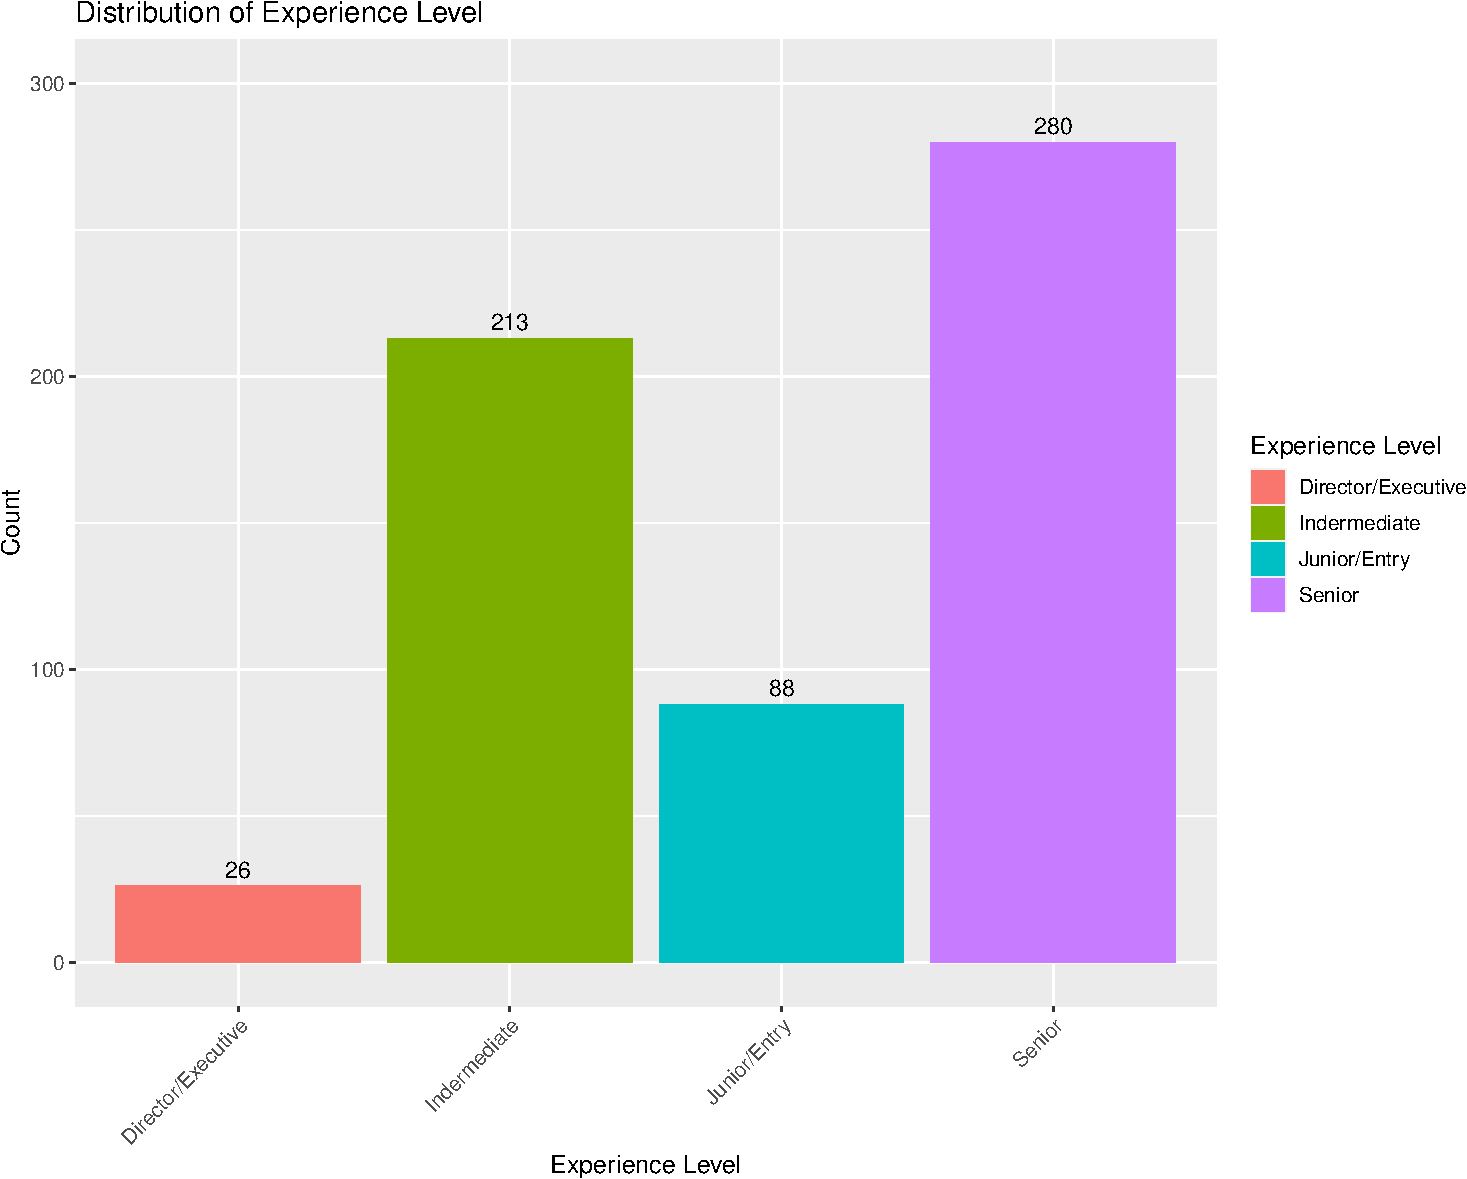
\includegraphics{Susman_RProject_files/figure-latex/Analysis-1.pdf} Most
people with data science related jobs are Senior level.

\begin{Shaded}
\begin{Highlighting}[]
\FunctionTok{library}\NormalTok{(ggplot2)}
\FunctionTok{library}\NormalTok{(tidyr)}

\NormalTok{job\_titles }\OtherTok{\textless{}{-}} \FunctionTok{c}\NormalTok{(}\StringTok{"Data Engineer"}\NormalTok{, }\StringTok{"Data Scientist"}\NormalTok{, }\StringTok{"Data Analyst"}\NormalTok{, }\StringTok{"Machine Learning Engineer"}\NormalTok{, }\StringTok{"Analytics Engineer"}\NormalTok{, }\StringTok{"Data Architect"}\NormalTok{, }\StringTok{"Research Scientist"}\NormalTok{, }\StringTok{"Applied Scientist"}\NormalTok{, }\StringTok{"Data Science Manager"}\NormalTok{, }\StringTok{"Research Engineer"}\NormalTok{)}

\NormalTok{query }\OtherTok{\textless{}{-}}\NormalTok{ salary\_df }\SpecialCharTok{\%\textgreater{}\%}
  \FunctionTok{filter}\NormalTok{(job\_title }\SpecialCharTok{\%in\%}\NormalTok{ job\_titles) }\SpecialCharTok{\%\textgreater{}\%}
  \FunctionTok{group\_by}\NormalTok{(job\_title, experience\_level) }\SpecialCharTok{\%\textgreater{}\%}
  \FunctionTok{summarise}\NormalTok{(}\AttributeTok{Count =} \FunctionTok{n}\NormalTok{(), }\AttributeTok{.groups =} \StringTok{"drop"}\NormalTok{) }\SpecialCharTok{\%\textgreater{}\%}
  \FunctionTok{complete}\NormalTok{(}\AttributeTok{job\_title =}\NormalTok{ job\_titles, experience\_level, }\AttributeTok{fill =} \FunctionTok{list}\NormalTok{(}\AttributeTok{Count =} \DecValTok{0}\NormalTok{)) }\SpecialCharTok{\%\textgreater{}\%}
  \FunctionTok{arrange}\NormalTok{(}\FunctionTok{desc}\NormalTok{(Count))}

\FunctionTok{ggplot}\NormalTok{(query, }\FunctionTok{aes}\NormalTok{(}\AttributeTok{x =} \FunctionTok{reorder}\NormalTok{(job\_title, }\SpecialCharTok{{-}}\NormalTok{Count), }\AttributeTok{y =}\NormalTok{ Count, }\AttributeTok{fill =}\NormalTok{ experience\_level)) }\SpecialCharTok{+}
  \FunctionTok{geom\_bar}\NormalTok{(}\AttributeTok{stat =} \StringTok{"identity"}\NormalTok{, }\AttributeTok{position =} \StringTok{"dodge"}\NormalTok{) }\SpecialCharTok{+}
  \FunctionTok{geom\_text}\NormalTok{(}\FunctionTok{aes}\NormalTok{(}\AttributeTok{label =}\NormalTok{ Count, }\AttributeTok{group =}\NormalTok{ experience\_level), }\AttributeTok{position =} \FunctionTok{position\_dodge2}\NormalTok{(}\AttributeTok{preserve =} \StringTok{"single"}\NormalTok{, }\AttributeTok{width =} \FloatTok{0.9}\NormalTok{), }\AttributeTok{vjust =} \SpecialCharTok{{-}}\FloatTok{0.5}\NormalTok{, }\AttributeTok{size =} \FloatTok{2.5}\NormalTok{, }\AttributeTok{color =} \StringTok{"black"}\NormalTok{) }\SpecialCharTok{+}
  \FunctionTok{scale\_x\_discrete}\NormalTok{(}\AttributeTok{labels =}\NormalTok{ job\_titles) }\SpecialCharTok{+}
  \FunctionTok{theme}\NormalTok{(}\AttributeTok{axis.text.x =} \FunctionTok{element\_text}\NormalTok{(}\AttributeTok{angle =} \DecValTok{50}\NormalTok{, }\AttributeTok{hjust =} \DecValTok{1}\NormalTok{, }\AttributeTok{vjust =} \DecValTok{1}\NormalTok{), }\AttributeTok{text =} \FunctionTok{element\_text}\NormalTok{(}\AttributeTok{size =} \DecValTok{10}\NormalTok{)) }\SpecialCharTok{+}
  \FunctionTok{labs}\NormalTok{(}\AttributeTok{title =} \StringTok{"Experience Level / Job Title"}\NormalTok{, }\AttributeTok{subtitle =} \StringTok{"For the 10 most popular data science jobs"}\NormalTok{, }\AttributeTok{x =} \StringTok{"Job Title"}\NormalTok{, }\AttributeTok{y =} \StringTok{"Count"}\NormalTok{) }\SpecialCharTok{+}
  \FunctionTok{guides}\NormalTok{(}\AttributeTok{fill =} \FunctionTok{guide\_legend}\NormalTok{(}\AttributeTok{title =} \StringTok{"Experience Level"}\NormalTok{)) }\SpecialCharTok{+}
  \FunctionTok{coord\_flip}\NormalTok{() }\SpecialCharTok{+}
  \FunctionTok{coord\_cartesian}\NormalTok{(}\AttributeTok{ylim =} \FunctionTok{c}\NormalTok{(}\DecValTok{0}\NormalTok{, }\DecValTok{80}\NormalTok{))}
\end{Highlighting}
\end{Shaded}

\begin{verbatim}
## Coordinate system already present. Adding new coordinate system, which will
## replace the existing one.
\end{verbatim}

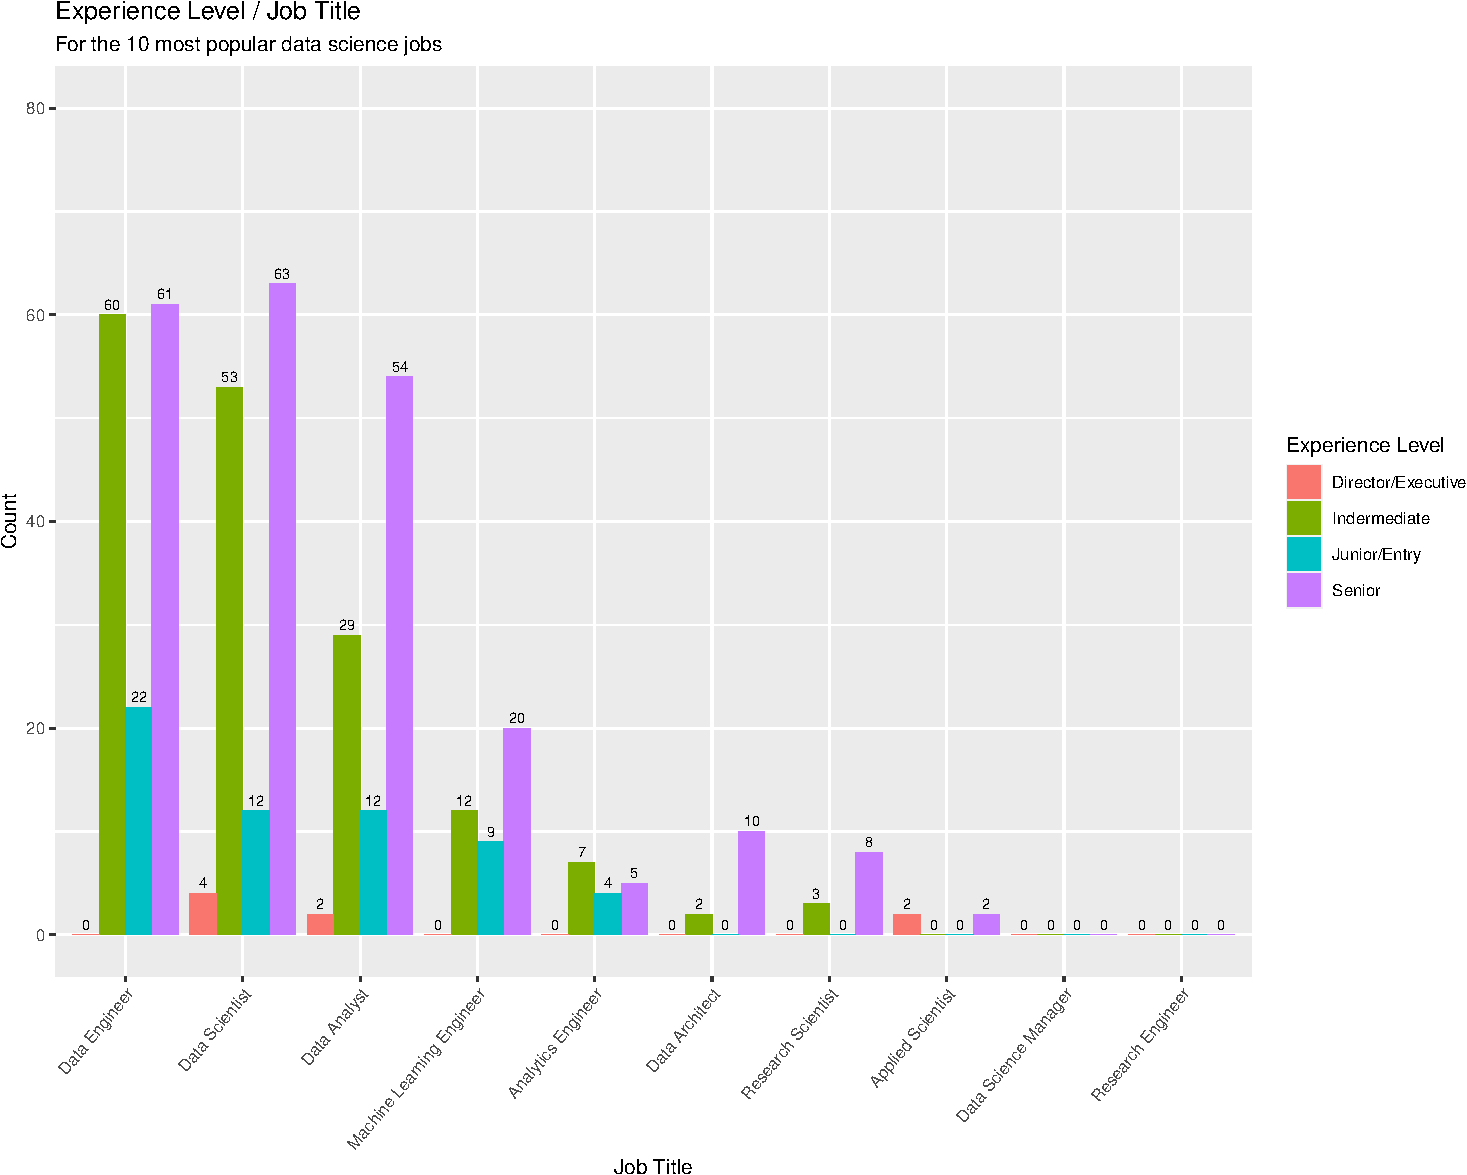
\includegraphics{Susman_RProject_files/figure-latex/unnamed-chunk-14-1.pdf}
The ratio of Seniors vs other experience levels is roughly the same per
job title.

\begin{Shaded}
\begin{Highlighting}[]
\FunctionTok{library}\NormalTok{(ggplot2)}

\NormalTok{employment\_type }\OtherTok{\textless{}{-}} \FunctionTok{data.frame}\NormalTok{(}\AttributeTok{employment\_type =}\NormalTok{ salary\_df}\SpecialCharTok{$}\NormalTok{employment\_type)}

\FunctionTok{ggplot}\NormalTok{(}\AttributeTok{data =}\NormalTok{ employment\_type, }\FunctionTok{aes}\NormalTok{(}\AttributeTok{x =}\NormalTok{ employment\_type)) }\SpecialCharTok{+}
  \FunctionTok{geom\_bar}\NormalTok{(}\AttributeTok{fill =} \StringTok{"orange"}\NormalTok{) }\SpecialCharTok{+}
  \FunctionTok{geom\_text}\NormalTok{(}\AttributeTok{stat =} \StringTok{"count"}\NormalTok{, }\FunctionTok{aes}\NormalTok{(}\AttributeTok{label =} \FunctionTok{after\_stat}\NormalTok{(count)), }\AttributeTok{vjust =} \SpecialCharTok{{-}}\FloatTok{0.5}\NormalTok{, }\AttributeTok{color =} \StringTok{"black"}\NormalTok{) }\SpecialCharTok{+}
  \FunctionTok{labs}\NormalTok{(}\AttributeTok{title =} \StringTok{"Employment Type Distribution"}\NormalTok{, }\AttributeTok{x =} \StringTok{"Employment Type"}\NormalTok{, }\AttributeTok{y =} \StringTok{"Count"}\NormalTok{) }\SpecialCharTok{+}
  \FunctionTok{theme}\NormalTok{(}\AttributeTok{axis.text.x =} \FunctionTok{element\_text}\NormalTok{(}\AttributeTok{angle =} \DecValTok{45}\NormalTok{, }\AttributeTok{hjust =} \DecValTok{1}\NormalTok{), }\AttributeTok{text =} \FunctionTok{element\_text}\NormalTok{(}\AttributeTok{size =} \DecValTok{14}\NormalTok{)) }\SpecialCharTok{+} 
  \FunctionTok{scale\_y\_continuous}\NormalTok{(}\AttributeTok{limits =} \FunctionTok{c}\NormalTok{(}\DecValTok{0}\NormalTok{, }\DecValTok{700}\NormalTok{))}
\end{Highlighting}
\end{Shaded}

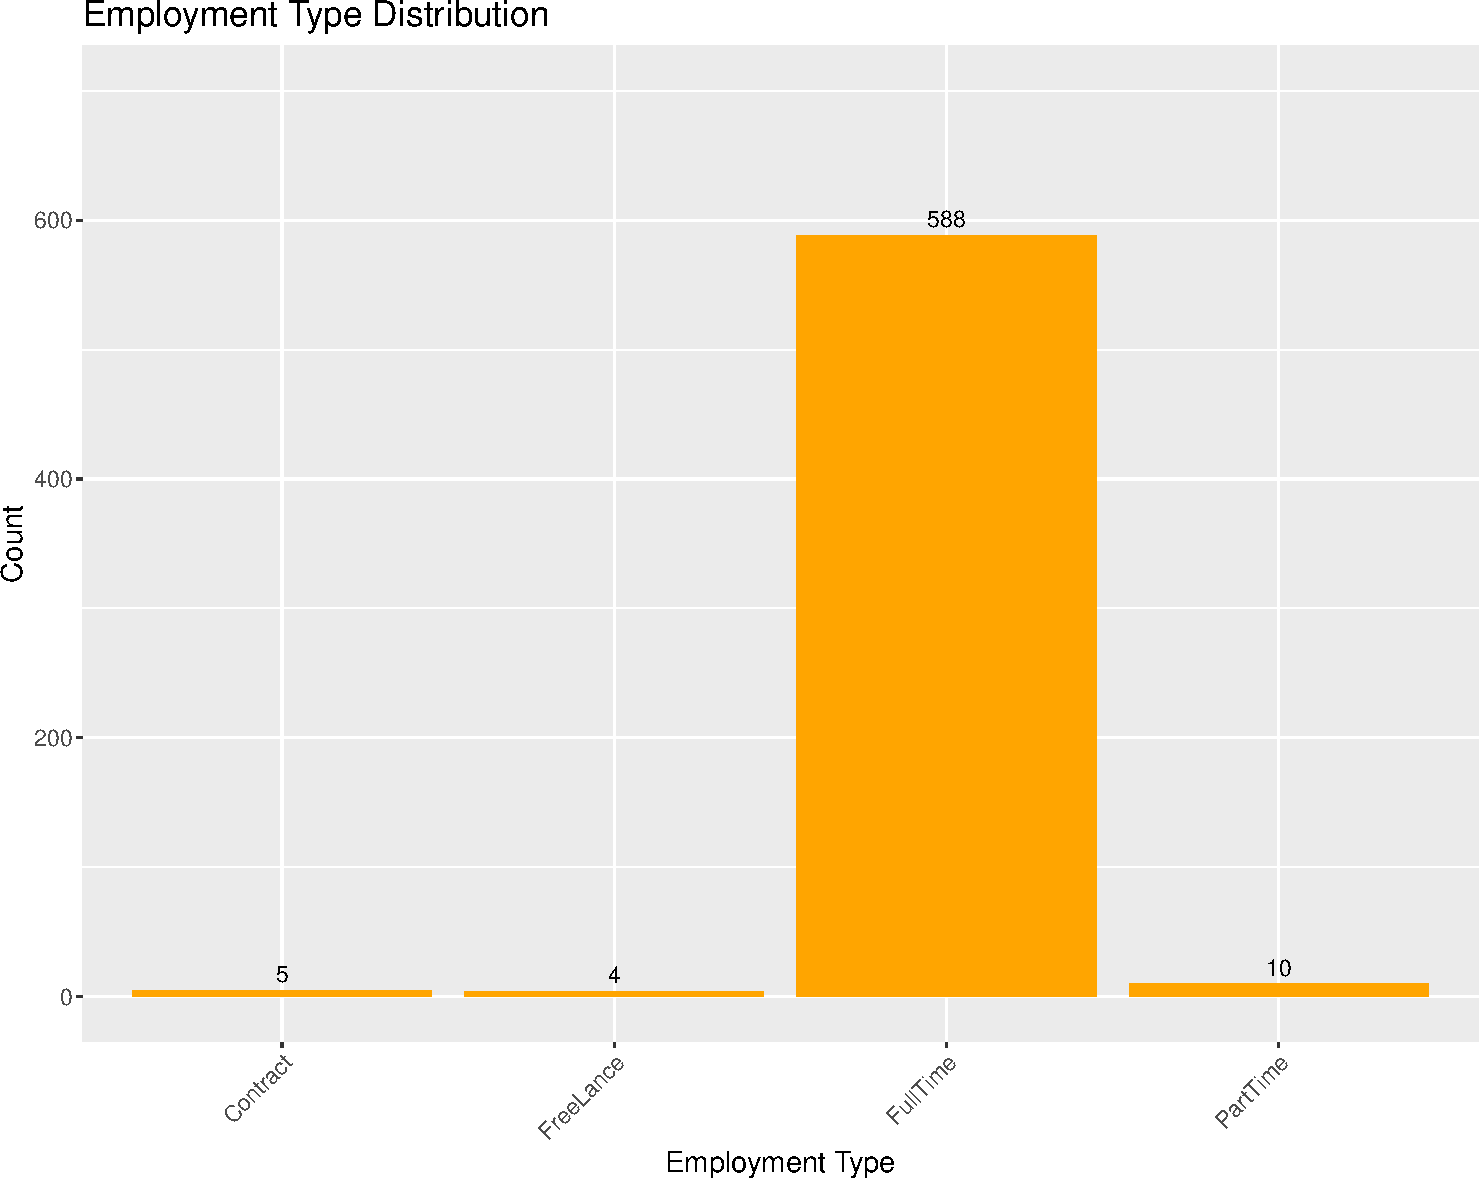
\includegraphics{Susman_RProject_files/figure-latex/unnamed-chunk-15-1.pdf}
Virtually all employees are full time.

\begin{Shaded}
\begin{Highlighting}[]
\NormalTok{job\_title\_counts }\OtherTok{\textless{}{-}} \FunctionTok{table}\NormalTok{(salary\_df}\SpecialCharTok{$}\NormalTok{job\_title)}

\CommentTok{\# Order the job titles in decreasing order}
\NormalTok{ordered\_counts }\OtherTok{\textless{}{-}} \FunctionTok{sort}\NormalTok{(job\_title\_counts, }\AttributeTok{decreasing =} \ConstantTok{TRUE}\NormalTok{)}

\CommentTok{\# Display the ordered job title counts}
\NormalTok{ordered\_counts}
\end{Highlighting}
\end{Shaded}

\begin{verbatim}
## 
##                           Data Scientist 
##                                      143 
##                            Data Engineer 
##                                      132 
##                             Data Analyst 
##                                       97 
##                Machine Learning Engineer 
##                                       41 
##                       Research Scientist 
##                                       16 
##                     Data Science Manager 
##                                       12 
##                           Data Architect 
##                                       11 
##                        Big Data Engineer 
##                                        8 
##               Machine Learning Scientist 
##                                        8 
##                             AI Scientist 
##                                        7 
##                   Data Analytics Manager 
##                                        7 
##                  Data Science Consultant 
##                                        7 
##                 Director of Data Science 
##                                        7 
##                 Principal Data Scientist 
##                                        7 
##                          BI Data Analyst 
##                                        6 
##                 Computer Vision Engineer 
##                                        6 
##                       Lead Data Engineer 
##                                        6 
##                              ML Engineer 
##                                        6 
##                   Applied Data Scientist 
##                                        5 
##                    Business Data Analyst 
##                                        5 
##                 Data Engineering Manager 
##                                        5 
##                             Head of Data 
##                                        5 
##                       Analytics Engineer 
##                                        4 
##       Applied Machine Learning Scientist 
##                                        4 
##                  Data Analytics Engineer 
##                                        4 
##                     Head of Data Science 
##                                        4 
##        Computer Vision Software Engineer 
##                                        3 
##                    Data Science Engineer 
##                                        3 
##                        Lead Data Analyst 
##                                        3 
##                      Lead Data Scientist 
##                                        3 
##               Machine Learning Developer 
##                                        3 
## Machine Learning Infrastructure Engineer 
##                                        3 
##                  Principal Data Engineer 
##                                        3 
##                      Cloud Data Engineer 
##                                        2 
##             Director of Data Engineering 
##                                        2 
##                            ETL Developer 
##                                        2 
##                   Financial Data Analyst 
##                                        2 
##                   Principal Data Analyst 
##                                        2 
##                     Product Data Analyst 
##                                        2 
##            3D Computer Vision Researcher 
##                                        1 
##                       Big Data Architect 
##                                        1 
##                      Data Analytics Lead 
##                                        1 
##                          Data Specialist 
##                                        1 
##                     Finance Data Analyst 
##                                        1 
##                 Head of Machine Learning 
##                                        1 
##           Lead Machine Learning Engineer 
##                                        1 
##                 Machine Learning Manager 
##                                        1 
##                   Marketing Data Analyst 
##                                        1 
##                             NLP Engineer 
##                                        1 
##                     Staff Data Scientist 
##                                        1
\end{verbatim}

\begin{Shaded}
\begin{Highlighting}[]
\FunctionTok{library}\NormalTok{(wordcloud)}
\end{Highlighting}
\end{Shaded}

\begin{verbatim}
## Loading required package: RColorBrewer
\end{verbatim}

\begin{Shaded}
\begin{Highlighting}[]
\DocumentationTok{\#\# Loading required package: RColorBrewer}
\FunctionTok{library}\NormalTok{(RColorBrewer)}

\CommentTok{\# Convert job\_title to character}
\NormalTok{salary\_df}\SpecialCharTok{$}\NormalTok{job\_title }\OtherTok{\textless{}{-}} \FunctionTok{as.character}\NormalTok{(salary\_df}\SpecialCharTok{$}\NormalTok{job\_title)}

\CommentTok{\# Filter the data based on job titles with count \textgreater{} 5}
\NormalTok{filtered\_counts }\OtherTok{\textless{}{-}}\NormalTok{ job\_title\_counts[job\_title\_counts }\SpecialCharTok{\textgreater{}} \DecValTok{5}\NormalTok{]}

\CommentTok{\# Generate 20 bright colors by repeating the "Set1" palette}
\NormalTok{num\_colors }\OtherTok{\textless{}{-}} \DecValTok{20}
\NormalTok{colors }\OtherTok{\textless{}{-}} \FunctionTok{rep}\NormalTok{(}\FunctionTok{brewer.pal}\NormalTok{(}\DecValTok{9}\NormalTok{, }\StringTok{"Set1"}\NormalTok{), }\AttributeTok{length.out =}\NormalTok{ num\_colors)}

\CommentTok{\# Create a data frame with word frequencies}
\NormalTok{word\_data }\OtherTok{\textless{}{-}} \FunctionTok{data.frame}\NormalTok{(}\AttributeTok{word =} \FunctionTok{names}\NormalTok{(filtered\_counts),}
                        \AttributeTok{freq =} \FunctionTok{as.numeric}\NormalTok{(filtered\_counts))}

\CommentTok{\# Set a dark background for the word cloud}
\FunctionTok{par}\NormalTok{(}\AttributeTok{bg =} \StringTok{"black"}\NormalTok{)}

\CommentTok{\# Generate the word cloud using wordcloud}
\FunctionTok{set.seed}\NormalTok{(}\DecValTok{123}\NormalTok{)  }\CommentTok{\# For reproducibility of colors and angles}
\FunctionTok{wordcloud}\NormalTok{(word\_data}\SpecialCharTok{$}\NormalTok{word, word\_data}\SpecialCharTok{$}\NormalTok{freq, }\AttributeTok{scale =} \FunctionTok{c}\NormalTok{(}\FloatTok{2.5}\NormalTok{, }\DecValTok{1}\NormalTok{), }\AttributeTok{random.order =} \ConstantTok{TRUE}\NormalTok{,}
          \AttributeTok{colors =}\NormalTok{ colors, }\AttributeTok{rot.per =} \FloatTok{0.2}\NormalTok{, }\AttributeTok{random.color =} \ConstantTok{TRUE}\NormalTok{)}
\end{Highlighting}
\end{Shaded}


\includegraphics{Susman_RProject_files/figure-latex/unnamed-chunk-17-1.pdf}

\begin{Shaded}
\begin{Highlighting}[]
\FunctionTok{library}\NormalTok{(ggplot2)}
\FunctionTok{library}\NormalTok{(dplyr)}

\CommentTok{\# Create a data frame with salary counts}
\NormalTok{salary }\OtherTok{\textless{}{-}}\NormalTok{ salary\_df }\SpecialCharTok{\%\textgreater{}\%}
  \FunctionTok{group\_by}\NormalTok{(salary\_in\_usd) }\SpecialCharTok{\%\textgreater{}\%}
  \FunctionTok{summarise}\NormalTok{(}\AttributeTok{count =} \FunctionTok{n}\NormalTok{())}

\CommentTok{\# Convert salary\_in\_usd to numeric}
\NormalTok{salary}\SpecialCharTok{$}\NormalTok{salary\_in\_usd }\OtherTok{\textless{}{-}} \FunctionTok{as.numeric}\NormalTok{(}\FunctionTok{as.character}\NormalTok{(salary}\SpecialCharTok{$}\NormalTok{salary\_in\_usd))}

\CommentTok{\# Sort the data frame by salary\_in\_usd}
\NormalTok{salary }\OtherTok{\textless{}{-}}\NormalTok{ salary[}\FunctionTok{order}\NormalTok{(salary}\SpecialCharTok{$}\NormalTok{salary\_in\_usd), ]}

\CommentTok{\# Set plot dimensions}
\FunctionTok{options}\NormalTok{(}\AttributeTok{repr.plot.width =} \DecValTok{15}\NormalTok{, }\AttributeTok{repr.plot.height =} \DecValTok{15}\NormalTok{)}

\CommentTok{\# Create the histogram plot with binwidth of 100000}
\FunctionTok{ggplot}\NormalTok{(salary, }\FunctionTok{aes}\NormalTok{(}\AttributeTok{x =}\NormalTok{ salary\_in\_usd)) }\SpecialCharTok{+}
  \FunctionTok{geom\_histogram}\NormalTok{(}\AttributeTok{binwidth =} \DecValTok{100000}\NormalTok{, }\AttributeTok{fill =} \StringTok{"lightblue"}\NormalTok{, }\AttributeTok{color =} \StringTok{"black"}\NormalTok{) }\SpecialCharTok{+}
  \FunctionTok{scale\_x\_continuous}\NormalTok{(}\AttributeTok{labels =}\NormalTok{ scales}\SpecialCharTok{::}\NormalTok{comma) }\SpecialCharTok{+}
  \FunctionTok{theme}\NormalTok{(}\AttributeTok{text =} \FunctionTok{element\_text}\NormalTok{(}\AttributeTok{size =} \DecValTok{20}\NormalTok{)) }\SpecialCharTok{+}
  \FunctionTok{labs}\NormalTok{(}\AttributeTok{title =} \StringTok{"Distribution of Salary"}\NormalTok{, }\AttributeTok{x =} \StringTok{"Salary"}\NormalTok{, }\AttributeTok{y =} \StringTok{"Count"}\NormalTok{)}
\end{Highlighting}
\end{Shaded}

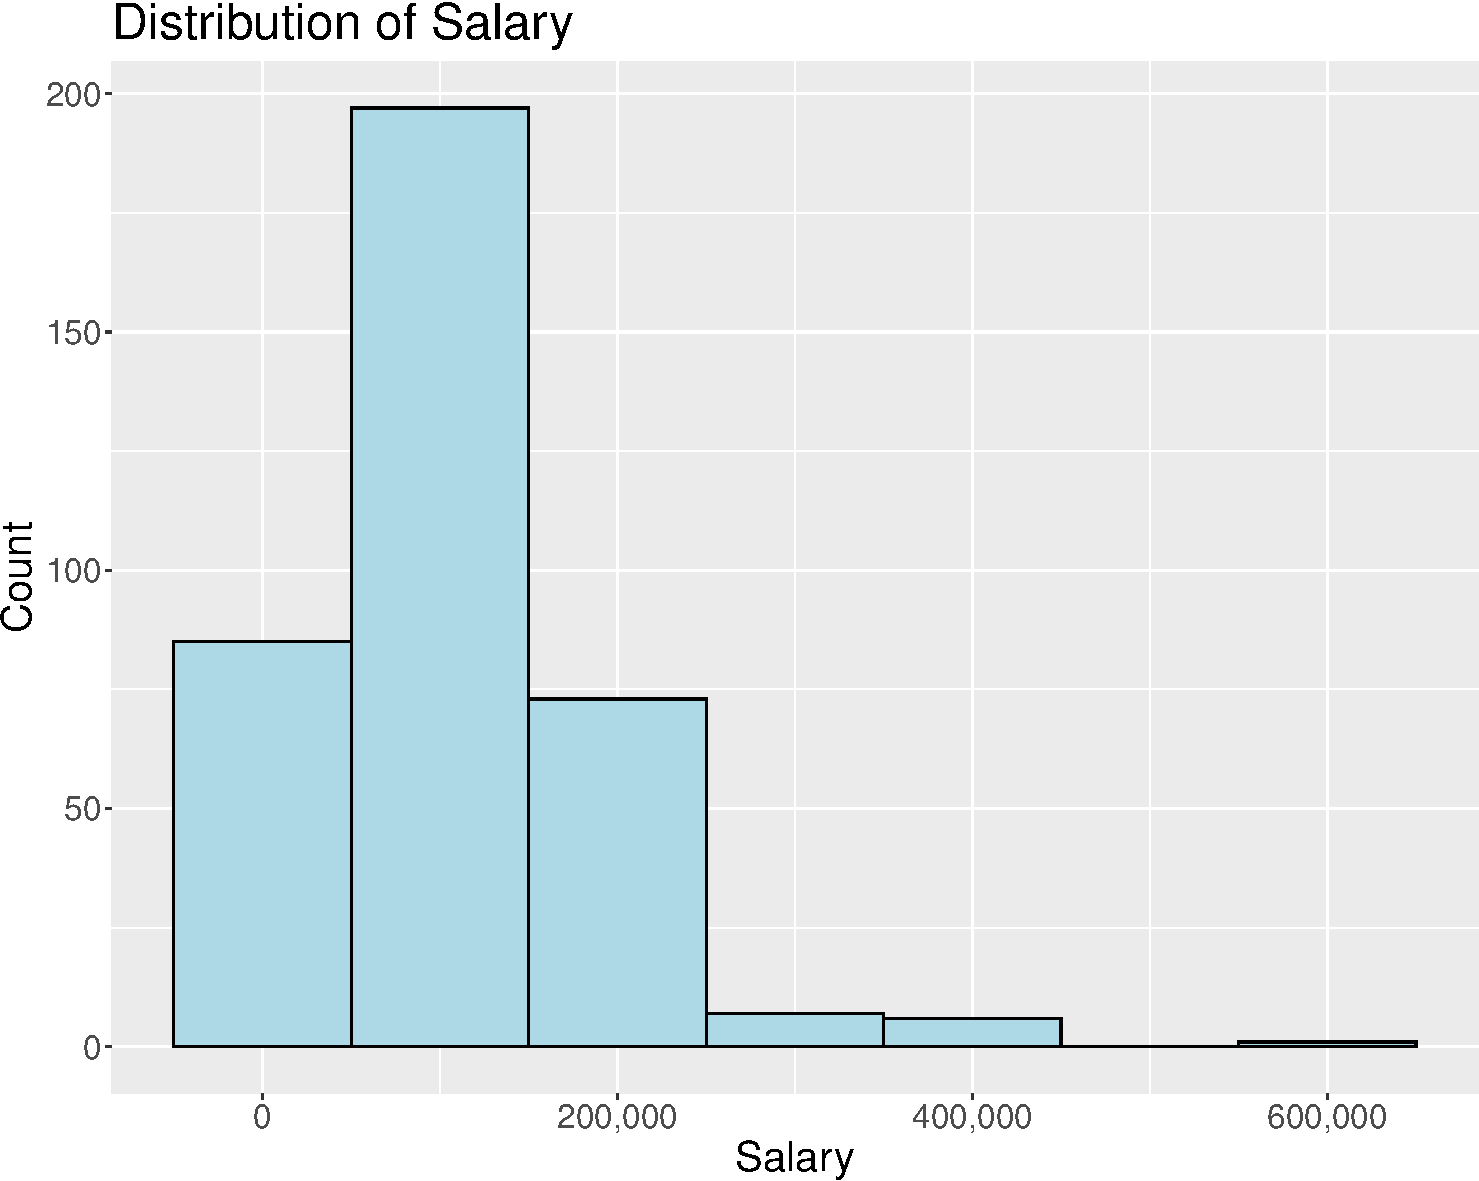
\includegraphics{Susman_RProject_files/figure-latex/unnamed-chunk-18-1.pdf}

\begin{Shaded}
\begin{Highlighting}[]
\CommentTok{\# Print summary statistics}
\FunctionTok{print}\NormalTok{(}\FunctionTok{summary}\NormalTok{(salary))}
\end{Highlighting}
\end{Shaded}

\begin{verbatim}
##  salary_in_usd        count       
##  Min.   :  2859   Min.   : 1.000  
##  1st Qu.: 53192   1st Qu.: 1.000  
##  Median : 93000   Median : 1.000  
##  Mean   :107471   Mean   : 1.645  
##  3rd Qu.:145000   3rd Qu.: 2.000  
##  Max.   :600000   Max.   :15.000
\end{verbatim}

\begin{Shaded}
\begin{Highlighting}[]
\FunctionTok{library}\NormalTok{(ggplot2)}
\FunctionTok{library}\NormalTok{(scales)}

\NormalTok{salary\_df}\SpecialCharTok{$}\NormalTok{salary\_in\_usd }\OtherTok{\textless{}{-}} \FunctionTok{as.numeric}\NormalTok{(salary\_df}\SpecialCharTok{$}\NormalTok{salary\_in\_usd)}

\NormalTok{temp }\OtherTok{\textless{}{-}} \FunctionTok{data.frame}\NormalTok{(}\FunctionTok{table}\NormalTok{(salary\_df}\SpecialCharTok{$}\NormalTok{job\_title))}

\NormalTok{temp }\OtherTok{\textless{}{-}}\NormalTok{ temp }\SpecialCharTok{\%\textgreater{}\%}
  \FunctionTok{arrange}\NormalTok{(}\FunctionTok{desc}\NormalTok{(Freq)) }\SpecialCharTok{\%\textgreater{}\%}
  \FunctionTok{head}\NormalTok{(}\AttributeTok{n =} \DecValTok{70}\NormalTok{)}

\NormalTok{data }\OtherTok{\textless{}{-}}\NormalTok{ salary\_df }\SpecialCharTok{\%\textgreater{}\%}
  \FunctionTok{select}\NormalTok{(job\_title, salary\_in\_usd) }\SpecialCharTok{\%\textgreater{}\%}
  \FunctionTok{filter}\NormalTok{(job\_title }\SpecialCharTok{==} \StringTok{"Data Engineer"} \SpecialCharTok{|}\NormalTok{ job\_title }\SpecialCharTok{==} \StringTok{"Data Scientist"} \SpecialCharTok{|}\NormalTok{ job\_title }\SpecialCharTok{==} \StringTok{"Data Analyst"} \SpecialCharTok{|}\NormalTok{ job\_title }\SpecialCharTok{==} \StringTok{"Machine Learning Engineer"} \SpecialCharTok{|}\NormalTok{ job\_title }\SpecialCharTok{==} \StringTok{"Analytics Engineer"} \SpecialCharTok{|}\NormalTok{ job\_title }\SpecialCharTok{==} \StringTok{"Data Architect"} \SpecialCharTok{|}\NormalTok{ job\_title }\SpecialCharTok{==} \StringTok{"Research Scientist"} \SpecialCharTok{|}\NormalTok{ job\_title }\SpecialCharTok{==} \StringTok{"Applied Scientist"} \SpecialCharTok{|}\NormalTok{ job\_title }\SpecialCharTok{==} \StringTok{"Data Science Manager"} \SpecialCharTok{|}\NormalTok{ job\_title }\SpecialCharTok{==} \StringTok{"Research Engineer"} \SpecialCharTok{|}\NormalTok{ job\_title }\SpecialCharTok{==} \StringTok{"ML Engineer"} \SpecialCharTok{|}\NormalTok{ job\_title }\SpecialCharTok{==} \StringTok{"Data Manager"} \SpecialCharTok{|}\NormalTok{ job\_title }\SpecialCharTok{==} \StringTok{"Machine Learning Scientist"} \SpecialCharTok{|}\NormalTok{ job\_title }\SpecialCharTok{==} \StringTok{"Data Science Consultant"} \SpecialCharTok{|}\NormalTok{ job\_title }\SpecialCharTok{==} \StringTok{"Data Analytics Manager"} \SpecialCharTok{|}\NormalTok{ job\_title }\SpecialCharTok{==} \StringTok{"Computer Vision Engineer"} \SpecialCharTok{|}\NormalTok{ job\_title }\SpecialCharTok{==} \StringTok{"AI Scientist"} \SpecialCharTok{|}\NormalTok{ job\_title }\SpecialCharTok{==} \StringTok{"BI Data Analyst"} \SpecialCharTok{|}\NormalTok{ job\_title }\SpecialCharTok{==} \StringTok{"Business Data Analyst"} \SpecialCharTok{|}\NormalTok{ job\_title }\SpecialCharTok{==} \StringTok{"Data Specialist"} \SpecialCharTok{|}\NormalTok{ job\_title }\SpecialCharTok{==} \StringTok{"BI Developer"} \SpecialCharTok{|}\NormalTok{ job\_title }\SpecialCharTok{==} \StringTok{"Applied Machine Learning Scientist"} \SpecialCharTok{|}\NormalTok{ job\_title }\SpecialCharTok{==} \StringTok{"AI Developer"} \SpecialCharTok{|}\NormalTok{ job\_title }\SpecialCharTok{==} \StringTok{"Big Data Engineer"} \SpecialCharTok{|}\NormalTok{ job\_title }\SpecialCharTok{==} \StringTok{"Director of Data Science"} \SpecialCharTok{|}\NormalTok{ job\_title }\SpecialCharTok{==} \StringTok{"Machine Learning Infrastructure Engineer"} \SpecialCharTok{|}\NormalTok{ job\_title }\SpecialCharTok{==} \StringTok{"Applied Data Scientist"} \SpecialCharTok{|}\NormalTok{ job\_title }\SpecialCharTok{==} \StringTok{"Data Operations Engineer"} \SpecialCharTok{|}\NormalTok{ job\_title }\SpecialCharTok{==} \StringTok{"ETL Developer"} \SpecialCharTok{|}\NormalTok{ job\_title }\SpecialCharTok{==} \StringTok{"Head of Data"}\NormalTok{)}

\FunctionTok{options}\NormalTok{(}\AttributeTok{repr.plot.width =} \DecValTok{15}\NormalTok{, }\AttributeTok{repr.plot.height =} \DecValTok{15}\NormalTok{)}

\NormalTok{data }\SpecialCharTok{\%\textgreater{}\%}
     \FunctionTok{ggplot}\NormalTok{(}\FunctionTok{aes}\NormalTok{(job\_title, salary\_in\_usd, }\AttributeTok{fill =}\NormalTok{ job\_title))}\SpecialCharTok{+}
     \FunctionTok{geom\_boxplot}\NormalTok{()}\SpecialCharTok{+}
     \FunctionTok{theme\_bw}\NormalTok{()}\SpecialCharTok{+}
     \FunctionTok{theme}\NormalTok{(}\AttributeTok{axis.text.x =} \FunctionTok{element\_text}\NormalTok{(}\AttributeTok{angle =} \DecValTok{90}\NormalTok{), }\AttributeTok{legend.position =} \StringTok{"none"}\NormalTok{, }\AttributeTok{text =} \FunctionTok{element\_text}\NormalTok{(}\AttributeTok{size =} \DecValTok{10}\NormalTok{))}\SpecialCharTok{+}
     \FunctionTok{scale\_y\_continuous}\NormalTok{(}\AttributeTok{labels =}\NormalTok{ comma)}\SpecialCharTok{+}
     \FunctionTok{labs}\NormalTok{(}\AttributeTok{title =} \StringTok{"Salary Range Based on Job Title for Data Science Jobs"}\NormalTok{, }\AttributeTok{subtitle =} \StringTok{"30 most popular data science jobs"}\NormalTok{, }\AttributeTok{x =} \StringTok{"Job Titles"}\NormalTok{, }\AttributeTok{y =} \StringTok{"Salary (USD)"}\NormalTok{)}
\end{Highlighting}
\end{Shaded}

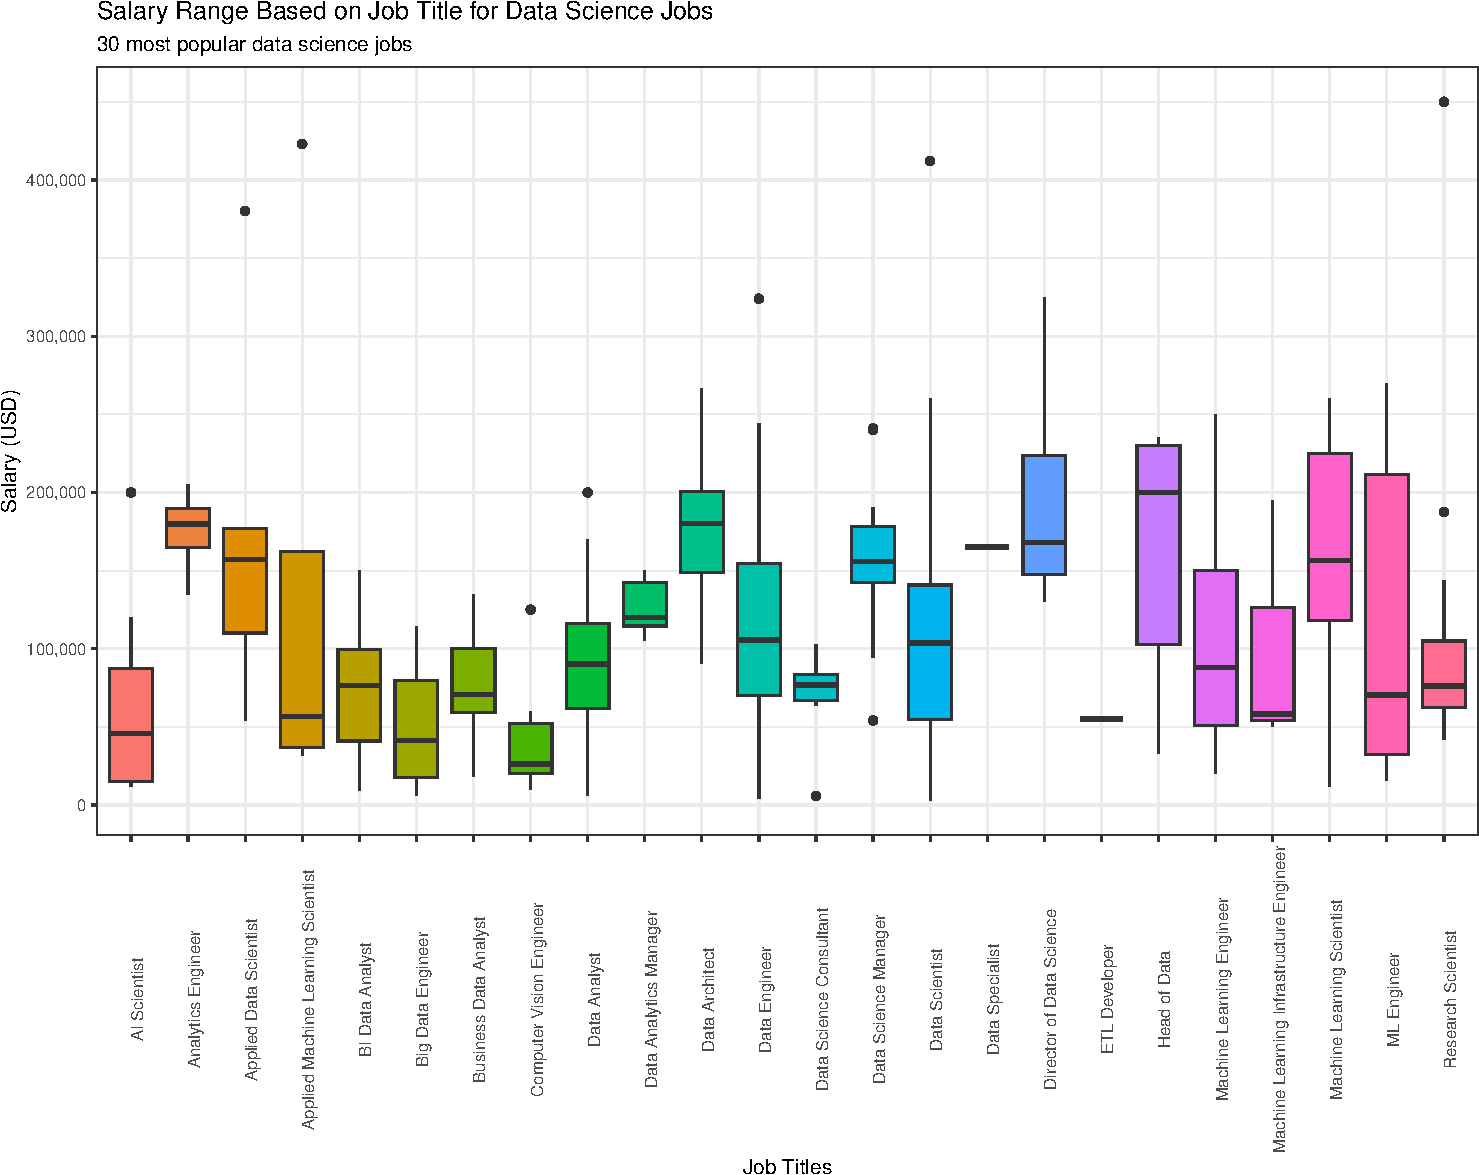
\includegraphics{Susman_RProject_files/figure-latex/unnamed-chunk-19-1.pdf}

\begin{Shaded}
\begin{Highlighting}[]
\FunctionTok{library}\NormalTok{(ggplot2)}
\FunctionTok{library}\NormalTok{(magrittr)}
\end{Highlighting}
\end{Shaded}

\begin{verbatim}
## 
## Attaching package: 'magrittr'
\end{verbatim}

\begin{verbatim}
## The following object is masked from 'package:purrr':
## 
##     set_names
\end{verbatim}

\begin{verbatim}
## The following object is masked from 'package:tidyr':
## 
##     extract
\end{verbatim}

\begin{Shaded}
\begin{Highlighting}[]
\NormalTok{remote\_ratio }\OtherTok{\textless{}{-}} \FunctionTok{data.frame}\NormalTok{(}\FunctionTok{table}\NormalTok{(salary\_df}\SpecialCharTok{$}\NormalTok{remote\_ratio))}

\FunctionTok{options}\NormalTok{(}\AttributeTok{repr.plot.width =} \DecValTok{15}\NormalTok{, }\AttributeTok{repr.plot.height =} \DecValTok{15}\NormalTok{)}

\NormalTok{remote\_ratio }\SpecialCharTok{\%\textgreater{}\%}
  \FunctionTok{ggplot}\NormalTok{() }\SpecialCharTok{+}
  \FunctionTok{aes}\NormalTok{(}\AttributeTok{x =}\NormalTok{ Var1, }\AttributeTok{y =}\NormalTok{ Freq) }\SpecialCharTok{+}
  \FunctionTok{geom\_col}\NormalTok{(}\AttributeTok{fill =} \StringTok{"lightgreen"}\NormalTok{, }\AttributeTok{color =} \StringTok{"black"}\NormalTok{) }\SpecialCharTok{+}
  \FunctionTok{geom\_text}\NormalTok{(}\FunctionTok{aes}\NormalTok{(}\AttributeTok{label =}\NormalTok{ Freq), }\AttributeTok{vjust =} \SpecialCharTok{{-}}\FloatTok{0.5}\NormalTok{, }\AttributeTok{size =} \DecValTok{5}\NormalTok{) }\SpecialCharTok{+}
  \FunctionTok{xlab}\NormalTok{(}\StringTok{"Remote Ratio"}\NormalTok{) }\SpecialCharTok{+}
  \FunctionTok{ylab}\NormalTok{(}\StringTok{"Count"}\NormalTok{) }\SpecialCharTok{+}
  \FunctionTok{ylim}\NormalTok{(}\FunctionTok{c}\NormalTok{(}\DecValTok{0}\NormalTok{, }\DecValTok{500}\NormalTok{)) }\SpecialCharTok{+}  \CommentTok{\# Set y{-}axis limits (adjust the upper limit as desired)}
  \FunctionTok{theme}\NormalTok{(}\AttributeTok{text =} \FunctionTok{element\_text}\NormalTok{(}\AttributeTok{size =} \DecValTok{16}\NormalTok{)) }\SpecialCharTok{+}
  \FunctionTok{labs}\NormalTok{(}\AttributeTok{title =} \StringTok{"Distribution of Remote Ratio"}\NormalTok{) }\SpecialCharTok{+}
  \FunctionTok{theme}\NormalTok{(}\AttributeTok{plot.margin =} \FunctionTok{margin}\NormalTok{(}\DecValTok{10}\NormalTok{, }\DecValTok{10}\NormalTok{, }\DecValTok{10}\NormalTok{, }\DecValTok{10}\NormalTok{, }\StringTok{"pt"}\NormalTok{))}
\end{Highlighting}
\end{Shaded}

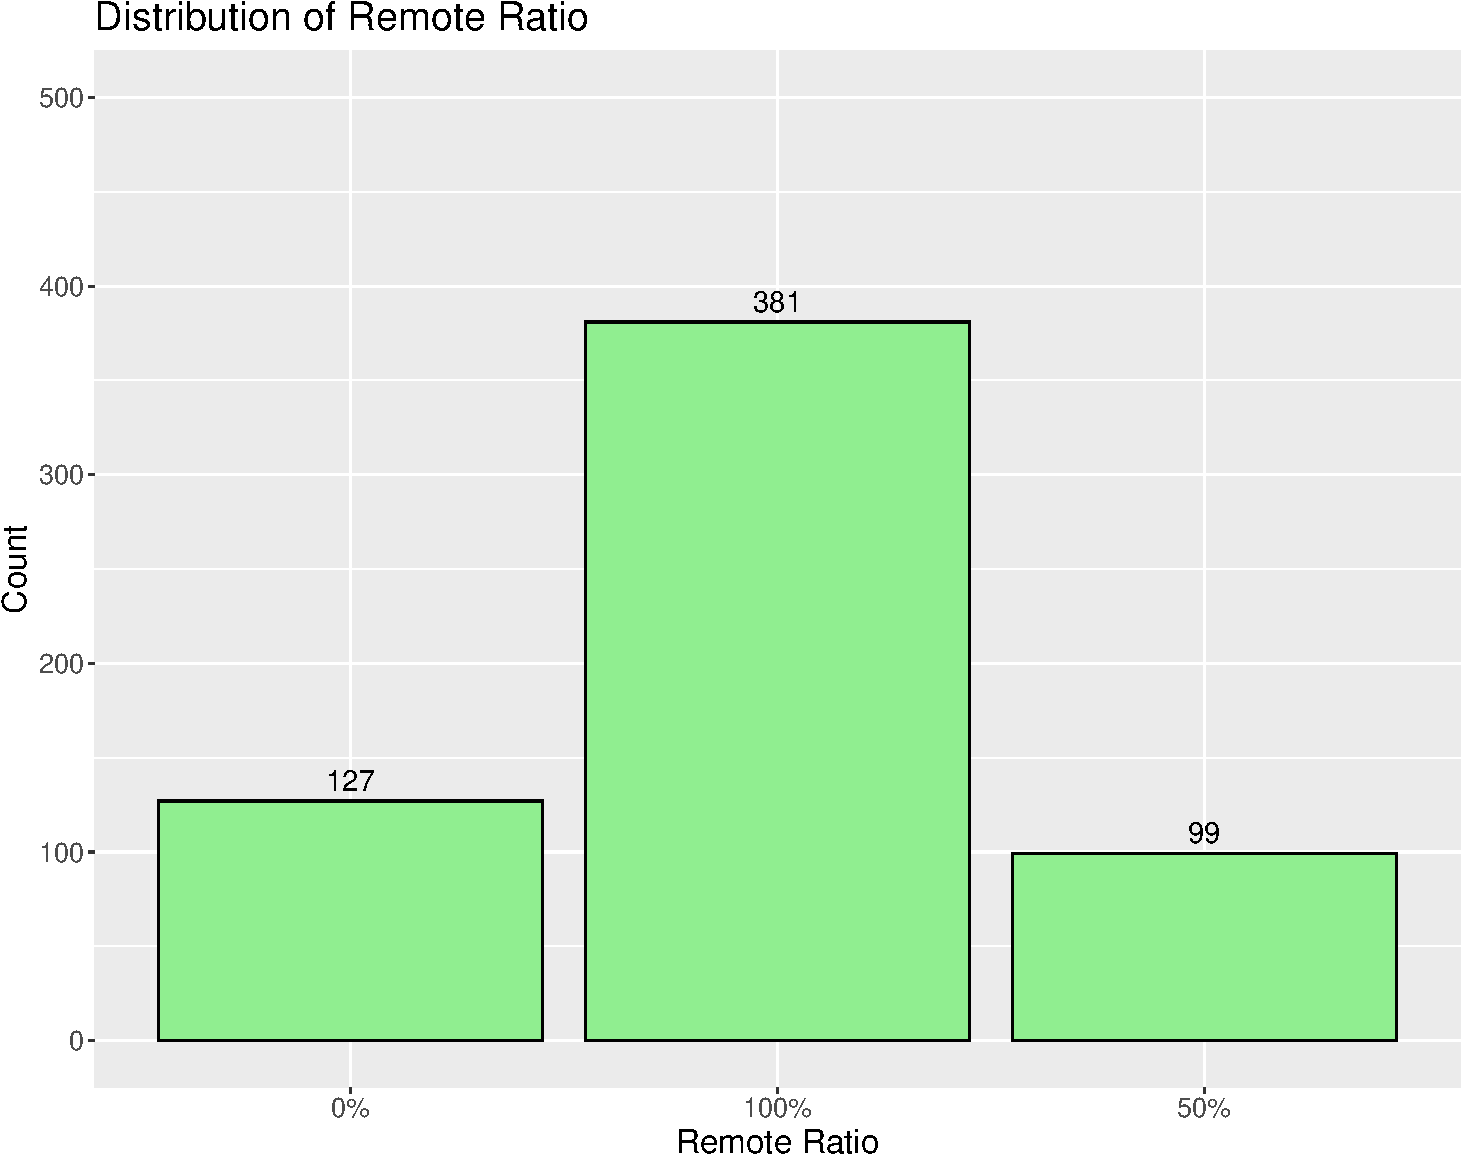
\includegraphics{Susman_RProject_files/figure-latex/unnamed-chunk-20-1.pdf}

\begin{Shaded}
\begin{Highlighting}[]
\NormalTok{company\_size }\OtherTok{\textless{}{-}} \FunctionTok{data.frame}\NormalTok{(}\FunctionTok{table}\NormalTok{(salary\_df}\SpecialCharTok{$}\NormalTok{company\_size))}

\FunctionTok{options}\NormalTok{(}\AttributeTok{repr.plot.width =} \DecValTok{15}\NormalTok{, }\AttributeTok{repr.plot.height =} \DecValTok{15}\NormalTok{)}

\NormalTok{ company\_size }\SpecialCharTok{\%\textgreater{}\%}
    \FunctionTok{ggplot}\NormalTok{() }\SpecialCharTok{+}
    \FunctionTok{aes}\NormalTok{(}\AttributeTok{x =}\NormalTok{ Var1, }\AttributeTok{y =}\NormalTok{ Freq) }\SpecialCharTok{+}
    \FunctionTok{geom\_col}\NormalTok{(}\AttributeTok{fill =} \StringTok{"purple"}\NormalTok{, }\AttributeTok{color =} \StringTok{"black"}\NormalTok{) }\SpecialCharTok{+}
    \FunctionTok{geom\_text}\NormalTok{(}\FunctionTok{aes}\NormalTok{(}\AttributeTok{label =}\NormalTok{ Freq), }\AttributeTok{vjust =} \SpecialCharTok{{-}}\FloatTok{0.5}\NormalTok{, }\AttributeTok{size =} \DecValTok{5}\NormalTok{) }\SpecialCharTok{+}
    \FunctionTok{labs}\NormalTok{(}\AttributeTok{title =} \StringTok{"Company Size Distribution"}\NormalTok{, }\AttributeTok{x =} \StringTok{"Company Size"}\NormalTok{, }\AttributeTok{y =} \StringTok{"Count"}\NormalTok{) }\SpecialCharTok{+}
    \FunctionTok{ylim}\NormalTok{(}\FunctionTok{c}\NormalTok{(}\DecValTok{0}\NormalTok{, }\DecValTok{450}\NormalTok{)) }\SpecialCharTok{+}  \CommentTok{\# Set y{-}axis limits (adjust the upper limit as desired)}
    \FunctionTok{theme}\NormalTok{(}\AttributeTok{text =} \FunctionTok{element\_text}\NormalTok{(}\AttributeTok{size =} \DecValTok{16}\NormalTok{)) }\SpecialCharTok{+}
    \FunctionTok{theme}\NormalTok{(}\AttributeTok{plot.margin =} \FunctionTok{margin}\NormalTok{(}\DecValTok{10}\NormalTok{, }\DecValTok{10}\NormalTok{, }\DecValTok{10}\NormalTok{, }\DecValTok{10}\NormalTok{, }\StringTok{"pt"}\NormalTok{))}
\end{Highlighting}
\end{Shaded}

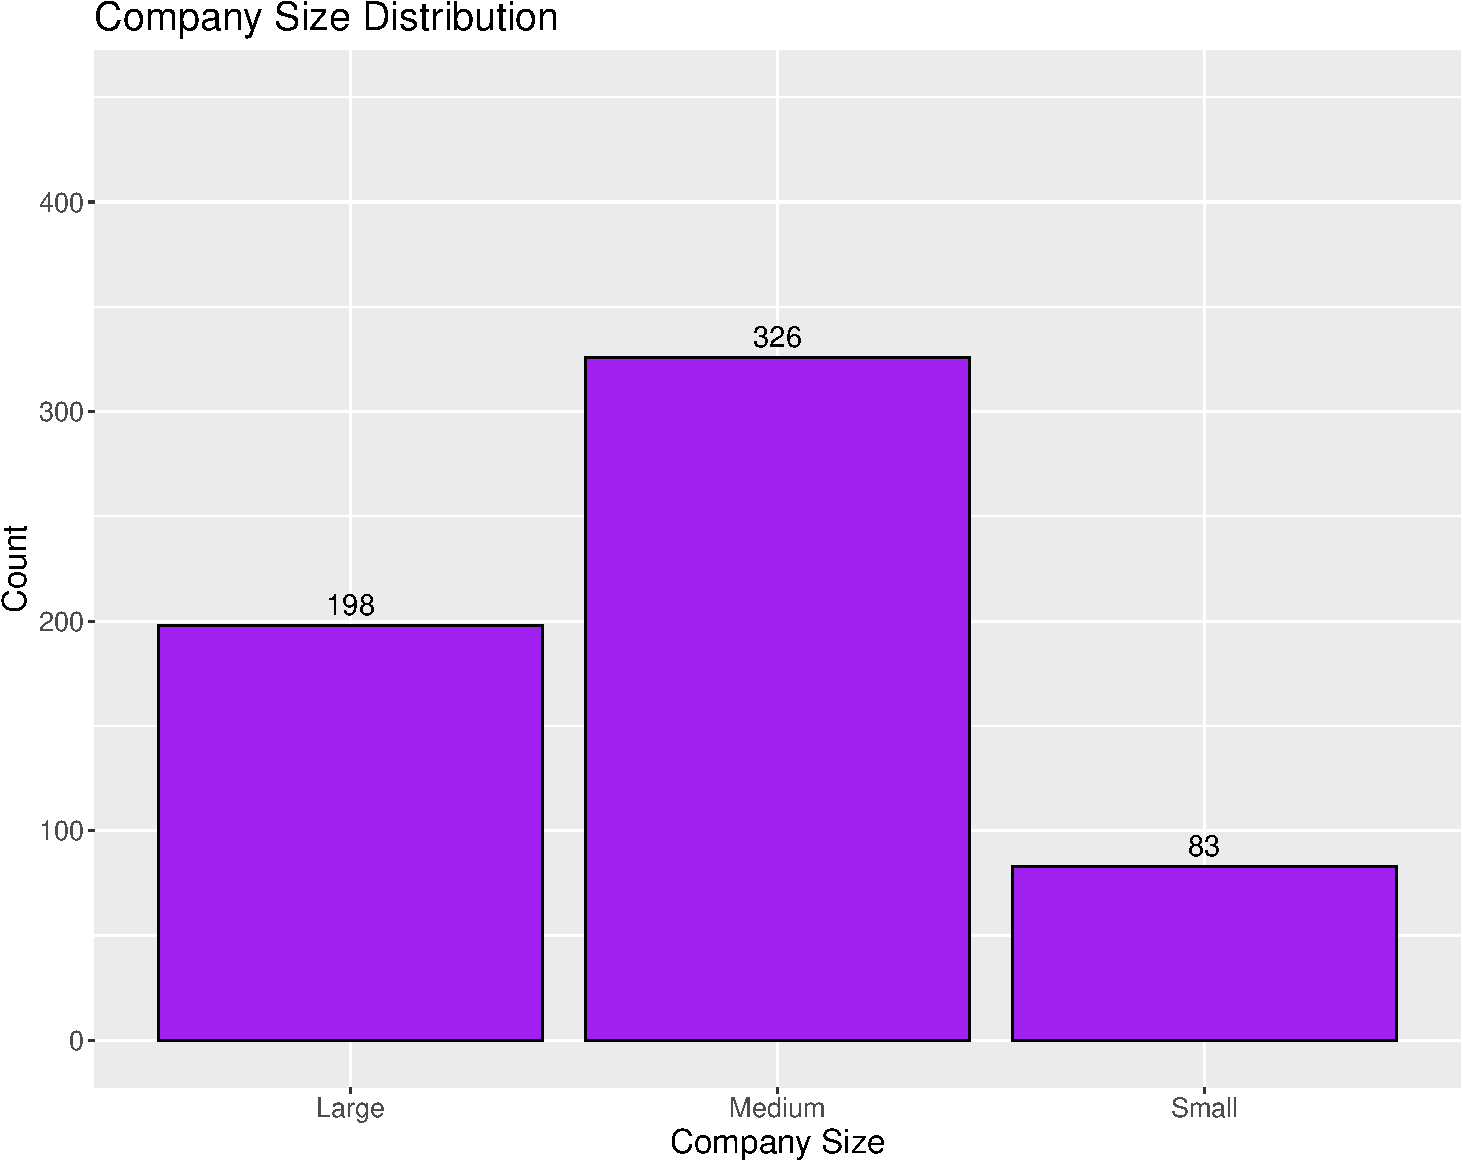
\includegraphics{Susman_RProject_files/figure-latex/unnamed-chunk-21-1.pdf}
Conclusion: In this analysis, I explored the salaries of data science
jobs in the US. I identified some trends and patterns in the data
science job market, such as most employee's experience being
senior-level and most data science companies are located in the US with
company sizes ranging from 50-250 employees. In conclusion, my analysis
provides a valuable snapshot of the current state and trends of data
science salaries in the US, which can help data scientists and employers
make informed decisions and plan their careers.

\end{document}
